% =================================================================== %
%   Tesis (template)
% =================================================================== %
%
%\documentclass[12pt,twoside,draft]{book}
\documentclass[12pt,twoside]{book}

% la opci�n draft es bueno activarla mientras uno est� escribiendo y despu�s hay que sacarla para la versi�n final 

% packages LaTeX adicionales
\usepackage[spanish]{babel}
\usepackage{amsmath}
\usepackage{amstext}
\usepackage{mathtools} 
\usepackage{amssymb}
\usepackage{longtable}
\usepackage{makeidx}
%\usepackage[dvips]{graphicx}
\usepackage{graphicx}
\graphicspath{ {./images/} }


\def\setbmp#1#2#3#4{\vskip#3\relax\noindent\hskip#1\relax
 \special{bmp:#4 x=#2, y=#3}}
\def\centerbmp#1#2#3{\vskip#2\relax\centerline{\hbox to#1{\special
  {bmp:#3 x=#1, y=#2}\hfil}}}


% idioma espa�ol
\selectlanguage{spanish}

% m�rgenes
\setlength{\textwidth}{150mm}
\setlength{\oddsidemargin}{9.6mm}
\setlength{\evensidemargin}{-0.6mm}
\setlength{\textheight}{217mm}
\setlength{\topmargin}{-5.4mm}
\setlength{\headheight}{10mm}
\setlength{\headsep}{10mm}

% doble espaciado entre lineas
\def\baselinestretch{1.30}

% profundidad en la tabla de contenidos
\setcounter{tocdepth}{2}

% hasta donde pone n�meros en el seccionado (ej 1.3.4.1)
\setcounter{secnumdepth}{4}

% definiciones de comandos especiales
%--------------------------------------------------------------------------
% Comandos usados en la tesis
%--------------------------------------------------------------------------


%--------------------------------------------------------------------------
% Definiciones de ambientes
%--------------------------------------------------------------------------
\newtheorem{defx}{Definici\'on}[chapter]
\newtheorem{lemx}{Lema}[chapter]
\newtheorem{corox}{Corolario}[chapter]
\newtheorem{algx}{Algoritmo}[chapter]
\newtheorem{ejemx}{Ejemplo}[chapter]
\newtheorem{propx}{Proposici\'on}[chapter]
\newtheorem{teox}{Teorema}[chapter]
\newtheorem{obsx}{Observaci\'on}[chapter]


\newenvironment{defi}[1]
    {\begin{defx}\rm(\emph{#1})\\}
    {\hfill $\blacksquare$ \end{defx}}

\newenvironment{ejem}
    {\begin{ejemx}\setlength{\parindent}{0pt}\rm}
    {\hfill $\blacksquare$ \end{ejemx}}

\newenvironment{alg}
    {\begin{algx}\begin{rm}}
    {\noindent \end{rm}\end{algx}}

\newenvironment{dem}
    {\textbf{Demostraci\'on:} \rm}
    {\hfill $\square$}\medskip

\newenvironment{lema}
    {\begin{lemx}\rm}
    {\hfill $\blacksquare$ \end{lemx}}

\newenvironment{obser}
    {\begin{obsx}\rm}
    {\hfill $\blacksquare$ \end{obsx}}

\newenvironment{prop}
    {\begin{propx}\rm}
    {\hfill $\blacksquare$ \end{propx}}

\newenvironment{coro}
    {\begin{corox}\rm}
    {\hfill $\blacksquare$ \end{corox}}

\newenvironment{teo}
    {\begin{teox}\rm}
    {\hfill $\blacksquare$ \end{teox}}

\newenvironment{obs}
    {\noindent {\textsc{Observaci\'on:\ }}}
    {}

%--------------------------------------------------------------------------
% Algunas siglas
%--------------------------------------------------------------------------
\newcommand{\TMS}{{\small TMS}}
\newcommand{\MTDR}{{\small MTDR}}
\newcommand{\PLR}{{\small PLR}}
\newcommand{\PLRO}{{\small PLRO}}
\newcommand{\SAA}{{\small SAA}}
\newcommand{\OSCAR}{{\small OSCAR}}
%--------------------------------------------------------------------------
% Comandos �tiles
%--------------------------------------------------------------------------

\newcommand{\tab}{\hspace*{1cm}}
\newcommand{\true}{\mbox{\textsc{true}}}
\newcommand{\false}{\mbox{\textsc{false}}}


\makeindex
% =================================================================== %

\begin{document}

\nocite{*}

\frontmatter\pagestyle{empty}

\begin{titlepage}
\begin{titlepage}

\begin{center}

\includegraphics[width=3cm,height=3cm]{uni.png}
\end{center}

\begin{center}

\textbf{\LARGE Universidad Nacional del Sur}\\

\vspace{2cm}

\textsc{\LARGE Proyecto Final de Carrera}\\ \vspace{.1cm}
\textsc{\LARGE Ingenier\'ia en Computaci\'on}\\


\vspace{4cm}

\emph{\LARGE Seguridad en redes LAN: utilizando Docker para mejorar la navegación web.}\\

\vspace{2.5cm}

{\Large Salvador Catalfamo}\\

\vspace{2.5cm}

{\sc\Large Bah\'{\i}a Blanca -- Argentina}\\
\vspace*{.1cm} {\Large 2021}

\end{center}
\end{titlepage}

\end{titlepage}

\begin{titlepage}
\begin{titlepage}

\begin{center}

\includegraphics[width=3cm,height=3cm]{uni.png}
\end{center}

\begin{center}

\textbf{\LARGE Universidad Nacional del Sur}\\

\vspace{2cm}

\textsc{\LARGE Proyecto Final de Carrera}\\ \vspace{.1cm}
\textsc{\LARGE Ingenier\'ia en Computaci\'on}\\


\vspace{4cm}

\emph{\LARGE Seguridad en redes LAN: utilizando Docker para mejorar la navegación web.}\\

\vspace{2.5cm}

{\Large Salvador Catalfamo}\\

\vspace{2.5cm}

{\sc\Large Bah\'{\i}a Blanca -- Argentina}\\
\vspace*{.1cm} {\Large 2021}

\end{center}
\end{titlepage}

\end{titlepage}


% =================================================================== %

% \setcounter{page}{1}

% resumen en castellano
\thispagestyle{empty}
\chapter*{Resumen}

% Aca va el resumen en castellano

\bigskip
A lo largo de la carrera, hemos visto como las organizaciones abordan los temas de seguridad en sus sistemas informáticos. Mayormente, se concentran en los equipos que están expuestos a la red pública, dejando de lado los que se encuentran aislados de la misma. Erróneamente, muchas veces se piensa que es suficiente, sin embargo, puede traer graves inconvenientes. Es por eso que realizaremos un estudio teórico/práctico sobre las consecuencias de la navegación en redes internas sin ningún tipo de cifrado de datos ni certificaciones.

\bigskip
\noindent \textsc{Palabras Clave:} \par

Seguridad e Infraestructura\par
Docker \par
Linux \par
Kali \par
Máquinas Virtuales  \par




\tableofcontents

%\listoffigures

% =================================================================== %
\mainmatter\pagestyle{headings}


\chapter{Introducci\'on} \pagenumbering{arabic}
    \label{capIntro}

%-*- ES -*-
%----------------------------------------------------------------------
% capitulo 1: Introduccion
%----------------------------------------------------------------------
% Estructura del capitulo:
%
%----------------------------------------------------------------------


% se pone una introducci�n al tema en general

\section{Objetivos}

\begin{itemize}
 \item item 1
 \item item 2
\end{itemize}


\begin{verbatim}
 Este es un bien ambiente para 
poner codigo
\end{verbatim}



En \cite{Davis:1989} se \footnote{Esta es una nota al pie} ve...
\\
\textit{casa} \\
\emph{casa} \\
\texttt{casa} \\
\textsf{casa} \\
\textbf{casa} \\

\subsection{objetivos principales}

\subsubsection{particulares}

\begin{center}
\begin{figure}


\includegraphics[width=3cm,height=3cm]{uni.bmp}

\caption{Esta es la figura del escudo de la uns}
\end{figure}
\end{center}

\section{Plan de tesis y principales contribuciones}\label{secContribuciones}

\section{Trabajos previos relacionados}
% rese�ar los art�culos hechos en el contexto del trabajo de tesis si los hay



% =================================================================== %





\chapter{(Ajustar) ¿Qué circula por una red interna? } 
    \label{capImp}

\section{Introducción}
Network Technology is the key technology for a wide variety of applications such as
email, file transfer, web browsing, online transactions, form fill up for various governmental or private activities, cab booking, etc. However, there is a significant lack of
easy implementation of security methods for these applications. 
\section{Protocolos asociados a la web}
    \section{Protocolo HTTP}

El Protocolo de transferencia de hipertexto (HTTP) es un protocolo de 
solicitud/respuesta \emph{stateless} (sin estado) que utiliza semántica 
extensible y cargas útiles de mensajes autodescriptivos para una 
interacción flexible con sistemas basados en red.

   HTTP es un protocolo genérico para sistemas de información. Está 
   diseñado para ocultar los detalles de cómo se implementa un servicio 
   mostrando una interfaz a los clientes que es independiente de los 
   tipos de recursos proporcionados. Del mismo modo, los servidores 
   no necesitan conocer el propósito de cada cliente: una solicitud 
   HTTP puede aislada en vez de estar asociada con un tipo específico
    de cliente o una secuencia predeterminada de pasos de la aplicación.
     
    El resultado es un protocolo que se puede utilizar de forma eficaz 
     en muchos contextos diferentes y cuyas implementaciones pueden
      evolucionar a lo largo del tiempo.
   Una consecuencia de esta flexibilidad es que el protocolo no 
   se puede definir en términos de lo que ocurre detrás de la 
   interfaz: estamos limitados a definir la sintaxis de la comunicación, 
   los mensajes y el comportamiento esperado de los destinatarios. 
   Si la comunicación se considera de forma aislada, las acciones 
   exitosas deben reflejarse correspondientemente. Sin embargo, 
   dado que varios clientes pueden actuar en paralelo y quizás con
    propósitos cruzados, no podemos exigir que tales cambios sean 
    observables más allá del alcance de una única respuesta.
   
\subsection{Arquitectura}
HTTP fue creado para la arquitectura World Wide Web (WWW) y ha 
evolucionado con el tiempo para soportar las necesidades de
 escalabilidad de un sistema mundial. Gran parte de esa arquitectura 
 se refleja en la terminología y  definiciones de sintaxis utilizadas 
 para definir HTTP.

\subsubsection*{Mensajes Cliente/Servidor}


HTTP es un protocolo de solicitud/respuesta que opera intercambiando 
mensajes a través de una ``conexión'' en la capa de sesión o transporte.
 Un “cliente” HTTP es un programa que establece una conexión a un 
 servidor con el propósito de enviar una o más solicitudes HTTP. 
 Un “servidor” HTTP es un programa que acepta conexiones para
  atender solicitudes HTTP mediante el envío de respuestas HTTP. 
  La mayoría de las comunicaciones HTTP consisten en una solicitud
   (GET) de algún recurso identificado por un URI. En el caso más 
   simple, esto podría lograrse mediante una única conexión entre un
    usuario y el servidor.

\begin{center}
   \begin{figure}   
      \begin{center}
         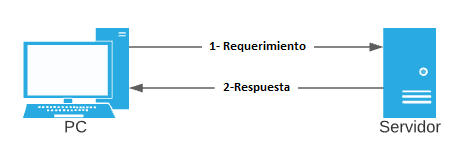
\includegraphics{2.1.png}
      \end{center}
      \caption{Comunicación básica en HTTP}
   \end{figure}
\end{center}

Un cliente envía una solicitud HTTP a un servidor en forma de mensaje
 de solicitud, comenzando con una línea que incluye un método, URI y 
 versión del protocolo, seguida de campos de encabezado que contienen
  modificadores de solicitud, información del cliente y metadatos de
   representación, una línea vacía para indicar el final de la sección
    del encabezado, y finalmente un cuerpo del mensaje que contiene el 
    cuerpo de la carga útil (si lo hay). 
    
    Un servidor responde a la 
    solicitud de un cliente enviando uno o más mensajes de respuesta 
    HTTP, cada uno de los cuales comienza con una línea de estado que 
    incluye la versión del protocolo, un código de estado (éxito o error)
     y una descripción en forma de texto asociada al mismo, posiblemente 
     seguida de campos de encabezado con información del servidor y
      metadatos de recursos, una línea vacía para indicar el final 
      de la sección del encabezado y finalmente, un cuerpo del mensaje
       la carga útil del mismo

\subsubsection*{Ejemplo}
El siguiente ejemplo ilustra un intercambio de mensajes típico 
para una solicitud GET a la dirección “http://www.example.com/hello.txt”:

\bigskip
\noindent
\underline{Client request:}
\begin{verbatim}
   GET /hello.txt HTTP/1.1
   User-Agent: curl/7.16.3 libcurl/7.16.3 OpenSSL/0.9.7l zlib/1.2.3
   Host: www.example.com
   Accept-Language: en, mi
  \end{verbatim}
\underline{Server response:}
\begin{verbatim}
   HTTP/1.1 200 OK
   Date: Mon, 27 Jul 2009 12:28:53 GMT
   Server: Apache
   Last-Modified: Wed, 22 Jul 2009 19:15:56 GMT
   ETag: "34aa387-d-1568eb00"
   Accept-Ranges: bytes
   Content-Length: 51
   Vary: Accept-Encoding
   Content-Type: text/plain

   Hello World! My payload includes a trailing CRLF.
\end{verbatim}


\subsection{Métodos mas importantes del del protocolo HTTP}

El protocolo HTTP contiene varios métodos, como por ejemplo PUT, HEAD, DELETE, etc. Sin
embargo, para nuestro trabajo explicaremos los dos mas utilizados GET y POST, lo que
nos permitirá tener una base a la hora de presentar el caso de estudio de la 
sección \ref{secCaseOfStudy}.

%CONNECT OPTIONS TRACE PUT 

\subsubsection*{GET}

El método GET solicita al servidor la transferencia de un recurso.
GET es el mecanismo principal de recuperación de información y el 
foco de casi todas las optimizaciones de rendimiento. Por lo tanto,
cuando las personas hablan de recuperar información identificable
a través de HTTP, generalmente se refieren a realizar una solicitud
GET.

Se puede pensar que a la hora de solicitar un recuro, este sea un archivo 
dentro de un directorio, y la respuesta sea el mismo archivo. Sin embargo, 
no existen tales limitaciones en la práctica. De hecho, se puede 
configurar un servidor para ejecutar los archivos de la solicitud y 
enviar la salida en lugar de transferir los archivos directamente. 
Independientemente de la solicitud, el servidor solo necesita saber 
cómo tratar a cada uno de sus recursos.

\subsubsection*{POST}

El método POST solicita que un recurso del servidor sea procesado con 
los datos que el cliente le envía. Por ejemplo, POST se utiliza para 
las siguientes funciones (entre otras):

\begin{itemize}
   \setlength\itemsep{-0.6em}
   \item Proporcionar un bloque de datos, como los campos ingresados 
   en un formulario HTML, a un proceso de manejo de datos.
   \item Publicar un mensaje grupo de 
   noticias, lista de correo, blog o grupo similar de artículos.
   \item Crear un nuevo recurso que aún no ha sido identificado por 
   el servidor.
   \item Agregar datos a las representaciones existentes de un recurso.
\end{itemize}


\subsection{Códigos de respuesta} 
El código de estado es un número entero de tres dígitos que da el 
resultado del intento de comprender y satisfacer la solicitud.
   Los códigos de estado HTTP son extensibles. No se requiere que los
    clientes HTTP comprendan el significado de todos los códigos de
     estado registrados, aunque se espera una mínima comprensión.

   Por ejemplo, si un cliente recibe un código de estado no reconocido
    de 471, el cliente puede asumir que hubo algo mal con su solicitud
     y tratar la respuesta como si hubiera recibido un código de estado
      400 (Solicitud incorrecta). El mensaje de respuesta generalmente 
      contendrá una representación que explica el estado.

   El primer dígito del código de estado define la clase de respuesta.
    Los dos últimos dígitos no tienen ninguna función de categorización.
     Hay cinco valores para el primer dígito:

   \begin{itemize}
      \setlength\itemsep{-0.6em}
      \item 1xx (Informativo): Se recibió la solicitud, se continua procesando.
      \item 2xx (Satisfactoria): La solicitud se recibió, comprendió y 
      aceptó correctamente.
      \item 3xx (Redireccionamiento): Se deben realizar más acciones para
    completar la solicitud.
    \item 4xx (Error del cliente): La solicitud contiene una sintaxis
    incorrecta o no se puede cumplir.
    \item 5xx (Error del servidor): El servidor no cumplió con una
       solicitud aparentemente válida.
   \end{itemize}

\subsection{Infraestructura de clave pública: una Introducción a la navegación segura (EL CONTENIDO 
VA A SER AGREGADO DESPUES DEL PRIMER FEEDBACK) }   

%
Gracias a la criptografía de clave pública, podemos comunicarnos de forma 
segura y confidencial con 
las personas cuyas claves públicas tengamos, pero hay una serie de problemas 
que siguen sin resolverse. Por ejemplo, ¿cómo podemos comunicarnos con personas que 
nunca hemos conocido? ¿Cómo almacenamos las claves públicas y las revocamos? Más 
importante aún, ¿cómo lo hacemos a escala mundial, con millones de servidores y 
miles de millones de personas y dispositivos? Es una tarea difícil, pero para eso 
se creó la infraestructura de clave pública (PKI).

El objetivo de PKI es permitir una comunicación segura entre partes que nunca se 
han conocido antes. El modelo que usamos hoy se basa en “trusted third parties” 
llamados autoridades de certificación (\emph{CA}, a veces también llamadas autoridades 
de certificación) para emitir certificados en los que confiamos siempre. Una 
infraestructura PKI está formado por los siguientes agentes.


\subsubsection*{Suscriptor}


El suscriptor (o entidad final) es la parte que desea brindar servicios 
seguros, que requieren un certificado. Por ejemplo: una empresa que desea 
publicar su sitio web.

\subsubsection*{Autoridad de Registro}

La autoridad de registro (RA) lleva a cabo determinadas funciones de gestión 
relacionadas con la emisión de certificados. Por ejemplo, una RA puede realizar 
la validación de identidad necesaria antes de solicitar a una \emph{CA} que emita un 
certificado. En algunos casos, las RA también se denominan autoridades de 
registro local (LRA). En la práctica, muchas \emph{CA} también realizan tareas de RA.

\subsubsection*{Autoridad de certificación}

Una autoridad de certificación (\emph{CA}) es un agente en el que confiamos para emitir 
certificados que confirman las identidades de los suscriptores. También están 
obligados a proporcionar información de revocación actualizada en línea para 
que las partes que confían puedan verificar que los certificados siguen siendo válidos.

\subsubsection*{Consumidor de certificados}

Técnicamente, se trata de los navegadores web, de programas y de sistemas 
operativos que realizan la validación de certificados. Para ello, contienen 
almacenes que contienen los certificados de confianza de algunas \emph{CA}. En un 
sentido más amplio, los agentes que confían son los usuarios finales que 
dependen de certificados para una comunicación segura en Internet.

\subsubsection*{Certificados}

Un certificado es un documento digital que contiene una clave pública, cierta 
información sobre la entidad asociada y una firma digital del emisor del 
certificado. En otras palabras, es una herramienta que nos permite intercambiar, 
almacenar y usar claves públicas. Con eso, los certificados se convierten en 
el componente básico de PKI.

\subsubsection*{Cadenas de certificados}

En la mayoría de los casos, un certificado de una entidad final por sí solo es 
insuficiente para una validación exitosa. En la práctica, cada servidor debe 
proporcionar una cadena de certificados que conduzca a una raíz de confianza. 
Las cadenas de certificados se utilizan por motivos de seguridad, técnicos y 
administrativos.

\subsubsection*{Autoridades de certificación}

Las autoridades de certificación (\emph{CA}) son la parte más importante del modelo 
actual de confianza en Internet. Pueden emitir un certificado para cualquier 
nombre de dominio, lo que significa que todo lo que digan es válido. 
Durante mucho tiempo, el costo de los certificados era bastante elevado. 
Sin embargo, en estos días, el precio se redujo drásticamente, impulsado 
por una fuerte competencia, adicionando a varias organizaciones que proveen 
estos servicios de manera gratuita. 

\subsubsection*{Ciclo de vida del certificado}

El ciclo de vida del certificado comienza cuando un suscriptor prepara una 
Solicitud de firma de certificado (CSR) y la envía a la \emph{CA} de su elección. 
El propósito principal del CSR es poner a disposición de la \emph{CA} la clave 
pública, así como demostrar la propiedad de la clave privada correspondiente 
(mediante una firma). 


\begin{center}
    \begin{figure}   
       \begin{center}
          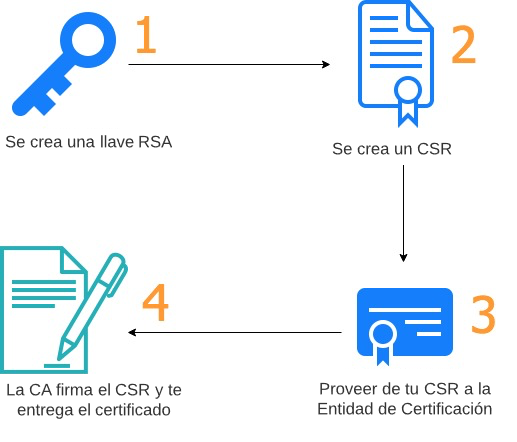
\includegraphics[width=9cm,height=8cm]{ca-process.png}
       \end{center}
       \caption{Solicitud de un certificado}
       \label{figSolCert}
    \end{figure}
 \end{center}



\subsection{HTTP con Seguridad SSL (HTTPS)} 

Con una comprensión mínima de los conceptos la criptografía, podemos 
observar cómo funciona el protocolo \emph{Secure Sockets Layer} (SSL). Aunque
 SSL no es un protocolo extremadamente complicado, ofrece varias 
 opciones y variaciones.

El protocolo SSL consiste en un conjunto de mensajes y reglas sobre
 cuándo enviar (y no enviar) cada mensaje. En esta sección, mostraremos 
 cuáles son esos mensajes, la información general que contienen y 
 cómo los sistemas usan los diferentes mensajes en una sesión de
  comunicaciones.


\subsubsection*{Roles SSL}
El protocolo \emph{Secure Sockets Layer} define dos roles diferentes para las
partes que se comunican. Por un lado tenemos un cliente, y por el otro
un servidor. La distinción es muy importante, porque SSL requiere que 
los dos sistemas se comporten de manera muy diferente. 

El cliente es el sistema que inicia las comunicaciones seguras; el 
servidor responde a la solicitud del cliente. En el uso más común 
de SSL, la navegación web segura, el navegador web es el cliente SSL 
y el sitio web es el servidor SSL. Para SSL en sí, las distinciones 
más importantes entre clientes y servidores son sus acciones durante 
la negociación de los parámetros de seguridad.

Dado que el cliente inicia una comunicación, tiene la responsabilidad 
de proponer un conjunto de opciones SSL para usar en el intercambio. 
El servidor selecciona entre las opciones propuestas por el cliente 
y decide qué utilizarán realmente los dos sistemas. Aunque la decisión 
final recae en el servidor, el servidor solo puede elegir entre las 
opciones que el cliente propuso originalmente.


\subsubsection*{Mensajes SSL}
Cuando los clientes y servidores SSL se comunican, lo hacen 
intercambiando mensajes SSL. Esta sección mostrará cómo los 
sistemas utilizan estos mensajes en sus comunicaciones. La función 
más básica (y uno de los propósitos mas importantes) que realiza 
un cliente y un servidor SSL es establecer la seguridad a través
de un canal para comunicaciones cifradas. Los primeros tres mensajes
SYN, SYN ACK y SYN correspondientes al protocolo TCP, Luego, inician los 
mensajes pertenecientes a la comunicación SSL.


\begin{center}
   \begin{figure}   
      \begin{center}
         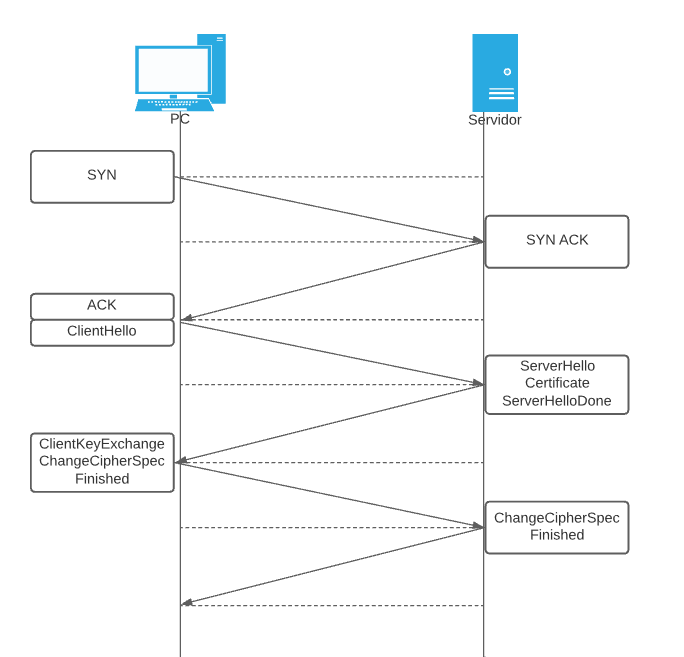
\includegraphics[width=13cm,height=13cm]{2.2.5.png}
      \end{center}
      \caption{Mensajes SSL}
   \end{figure}
\end{center}


\paragraph*{ClientHello}
El mensaje \emph{ClientHello} inicia la comunicación SSL entre las dos partes. 
El cliente usa este mensaje para pedirle al servidor que comience a 
negociar los servicios de seguridad usando SSL.

El mensaje este compuesto por ciertos campos: 
\begin{itemize}
   \setlength\itemsep{-0.6em}
   \item Versión: refiere a la versión más alta de SSL que el cliente 
   puede admitir. 
   \item RandomNumber: proporciona la semilla para cálculos criptográficos
   críticos. 
   \item SessionID: es opcional, y muchas veces no es utilizado. 
   \item CipherSuites: permite a un cliente enumerar los diversos 
   servicios criptográficos que el cliente puede admitir
   \item CompressionMethods: es utilizado por el cliente para enumerar 
   todos los diversos métodos de compresión de datos que puede admitir.
    Los métodos de compresión son una parte importante de SSL porque el 
    cifrado tiene una secuencia significativa en la efectividad de 
    cualquier técnica de compresión de datos. 
\end{itemize}


\paragraph*{ServerHello}
Este mensaje complementa el campo \emph{CipherSuite} del \emph{ServerHello}. Si bien 
el campo \emph{CipherSuite} indica los algoritmos criptográficos y los tamaños 
de clave, este mensaje contiene la información de la clave pública en sí. 
Tenga en cuenta que el mensaje \emph{ServerKeyExchange} se transmite sin cifrado, 
por lo que solo se puede incluir de forma segura información de clave 
pública. El cliente utilizará la clave pública del servidor para cifrar 
una clave de sesión, que las partes utilizarán para cifrar los datos de 
la aplicación para la sesión.

\paragraph*{ServerKeyExchange}

Este mensaje complementa el campo \emph{CipherSuite} del \emph{ServerHello}. 
Si bien el campo \emph{CipherSuite} indica los algoritmos criptográficos y 
los tamaños de clave, este mensaje contiene la información de la clave 
pública en sí. Tenga en cuenta que el mensaje \emph{ServerKeyExchange} se 
transmite sin cifrado, por lo que solo se puede incluir de forma 
segura información de clave pública. El cliente utilizará la clave 
pública del servidor para cifrar una clave de sesión, que las partes 
utilizarán para cifrar los datos de la aplicación para la sesión.

\paragraph*{ServerHelloDone}
El mensaje \emph{ServerHelloDone} le dice al cliente que el servidor ha 
terminado con sus mensajes iniciales de negociación. El mensaje en 
sí no contiene otra información, pero es importante para el cliente, 
porque una vez que el cliente recibe un \emph{ServerHelloDone}, puede pasar a 
la siguiente fase para establecer las comunicaciones seguras.

\paragraph*{ClientKeyExchange}
Cuando el servidor ha terminado su parte de la negociación SSL inicial, 
el cliente responde con un mensaje \emph{ClientKeyExchange}. Así como 
\emph{ServerKeyExchange} proporciona la información clave para el servidor, 
\emph{ClientKeyExchange} le dice al servidor la información clave del cliente. 
En este caso, sin embargo, la información clave es para el algoritmo de 
cifrado simétrico que ambas partes usarán para la sesión. Además, la 
información del mensaje del cliente se cifra mediante la clave pública 
del servidor. Este cifrado protege la información de la clave a medida 
que atraviesa la red y permite al cliente verificar que el servidor 
realmente posee la clave privada correspondiente a su clave pública. 
De lo contrario, el servidor no podrá descifrar este mensaje. Esta 
operación es una protección importante contra un atacante que intercepta 
mensajes de un servidor legítimo y finge ser ese servidor reenviando los 
mensajes a un cliente desprevenido. Dado que un servidor falso no conocerá 
la clave privada del servidor real, no podrá descifrar el mensaje 
\emph{ClientKeyExchange}. Sin la información en ese mensaje, la comunicación 
entre las dos partes no puede tener éxito.
\paragraph*{ChangeCipherSpec}
Una vez que el cliente envía información clave en un mensaje 
\emph{ClientKeyExchange}, se completa la negociación SSL preliminar. En ese 
momento, las partes están listas para comenzar a utilizar los servicios 
de seguridad que han negociado.

El protocolo SSL define un mensaje especial, \emph{ChangeCipherSpec}, para 
indicar explícitamente que ahora se deben invocar los servicios de 
seguridad. Un conjunto de claves protegerá los datos que el cliente 
envía al servidor, y un conjunto diferente de claves protegerá los 
datos que el servidor envía al cliente. Para cualquier sistema dado, 
ya sea un cliente o un servidor, SSL define un estado de escritura y 
un estado de lectura. El estado de escritura define la información de 
seguridad de los datos que envía el sistema y el estado de lectura 
define la información de seguridad de los datos que recibe el sistema.

\paragraph*{Finished}
Inmediatamente después de enviar sus mensajes \emph{ChangeCipherSpec}, cada 
sistema también envía un mensaje \emph{Finished}. Los mensajes \emph{Finished}
permiten que ambos sistemas verifiquen que la negociación se ha realizado 
correctamente y que la seguridad no se ha visto comprometida.

Cada mensaje \emph{Finished} contiene un hash criptográfico de información 
importante sobre la negociación recién finalizada. Esto protege contra 
un atacante que logra insertar mensajes ficticios o eliminar mensajes 
legítimos de la comunicación. Si un atacante pudiera hacerlo, los 
cálculos de hash del cliente y del servidor no coincidirían y detectarían 
el compromiso.

\paragraph*{Finalización de las comunicaciones seguras}

Aunque, en la práctica, rara vez se utiliza (principalmente debido a la 
naturaleza de las sesiones web), SSL tiene un procedimiento definido para 
finalizar una comunicación segura entre dos partes. En este procedimiento, 
los dos sistemas envían cada uno una alerta de cierre especial al otro. 
El cierre explícito de una sesión protege contra un ataque de truncamiento,
en el que un atacante puede comprometer la seguridad al terminar 
prematuramente una comunicación.

\subsubsection*{Autenticar la identidad del servidor}
Anteriormente se explicó cómo SSL puede establecer comunicaciones 
cifradas entre dos partes, lo que puede no agregar mucha seguridad a 
la comunicación. Con el cifrado solo, ninguna de las partes puede 
estar realmente segura de la identidad de la otra. La razón típica 
para usar el cifrado en primer lugar es mantener la información en 
secreto de algún tercero. Pero si ese tercero pudiera hacerse pasar 
con éxito como el destinatario previsto de la información, entonces el 
cifrado no serviría de nada. Los datos estarían encriptados, pero el 
atacante tendría todos los datos necesarios para desencriptarlos. Para 
evitar este tipo de ataques, SSL incluye mecanismos que permiten a cada 
parte autenticar la identidad de la otra. Con estos mecanismos, cada 
parte puede estar segura de que la otra es genuina y no un atacante 
enmascarado. En esta sección, veremos cómo SSL permite que un servidor 
se autentique.

\paragraph*{Certificate}
Al autenticar su identidad, el servidor envía un mensaje de certificado 
en lugar del mensaje \emph{ServerKeyExchange} descrito anteriormente. El mensaje 
\emph{Certificate} simplemente contiene una cadena de certificados que comienza 
con el certificado de clave pública del servidor y termina con el certificado 
raíz de la autoridad certificadora.

El cliente tiene la responsabilidad de asegurarse de que puede confiar 
en el certificado que recibe del servidor. Esa responsabilidad incluye 
verificar las firmas del certificado, los tiempos de validez y el estado 
de revocación. También significa asegurarse de que la autoridad de 
certificación sea una en la que el cliente confíe. Normalmente, los clientes 
toman esta determinación conociendo la clave pública de las autoridades de 
certificación confiables de antemano, a través de algunos medios confiables. 
Microsoft, por ejemplo, carga su software con claves públicas para 
autoridades de certificación conocidas.

\paragraph*{ClientKeyExchange}
El mensaje \emph{ClientKeyExchange} del cliente también difiere en la autenticación 
del servidor, aunque la diferencia no es importante. Cuando solo se va a 
utilizar cifrado, el cliente cifra la información en en mensaje 
\emph{ClientKeyExchange}
utilizando la clave pública que el servidor proporciona en su mensaje 
\emph{ServerKeyExchange}. En este caso, por supuesto, el servidor se está 
autenticando y, por lo tanto, ha enviado un mensaje de certificado en 
lugar de un \emph{ServerKeyExchange}. El cliente, por lo tanto, encripta su 
información usando la clave pública contenida en el 
certificado del servidor. Este paso es importante porque le permite 
al cliente asegurarse de que la parte con la que se está comunicando 
realmente posee la clave privada del servidor. Solo un sistema con la 
clave privada real podrá descifrar este mensaje y continuar con éxito 
la comunicación.

 

\subsubsection*{Niveles de validación}  
Hay tres tipos de certificados SSL disponibles en la actualidad: validación por 
dominio (DV),
validación por organización (OV) y validación extendida (EV).
Los niveles de cifrado son los mismos para cada certificado, lo que difiere son los 
procesos de investigación y verificación necesarios para obtener el certificado.

\paragraph*{Validación de dominio (DV)}
Validación de dominio SSL o DV SSL representa el nivel base para los tipos de SSL. 
Estos son perfectos para sitios web que solo necesitan cifrado y nada más. Los 
certificados DV SSL suelen ser económicos y se pueden emitir en cuestión de minutos. 
Eso es porque el proceso de validación está completamente automatizado. Simplemente 
es necesario demostrar que es propietario de su dominio y que el certificado DV 
es suyo. 

\begin{center}
   \begin{figure}   
      \begin{center}
         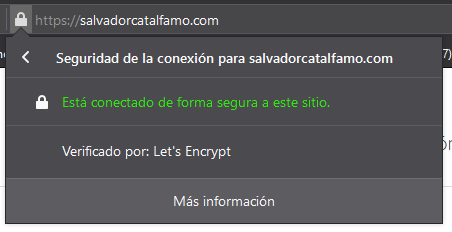
\includegraphics{dv.png}
      \end{center}
      \caption{Validación de dominio}
   \end{figure}
\end{center}

\paragraph*{Validación de la organización (OV)}
Validación de organización u OV SSL representa el término medio para los tipos de 
certificados SSL. Para obtener OV SSL, su empresa u organización debe someterse a 
un examen comercial ligero. Esto puede demorar hasta tres días hábiles porque alguien 
tiene que verificar la información de su empresa. OV SSL muestra los mismos indicadores 
visuales que DV SSL, pero proporciona una forma de ver la 
información comercial verificada en la sección de detalles del certificado. 

\paragraph*{Extended Validation (EV)}
SSL de validación extendida o SSL con EV requiere un exhaustivo examen comercial. 
Esto puede parecer mucho, pero en realidad no lo es si su empresa tiene 
registros disponibles públicamente. EV SSL activaba un indicador visual único: el 
nombre de su organización verificado que se muestra en el navegador. Esto en la 
actualidad ya no sucede, por lo que no es posible a simple vista identificarlo.

\begin{center}
   \begin{figure}   
      \begin{center}
         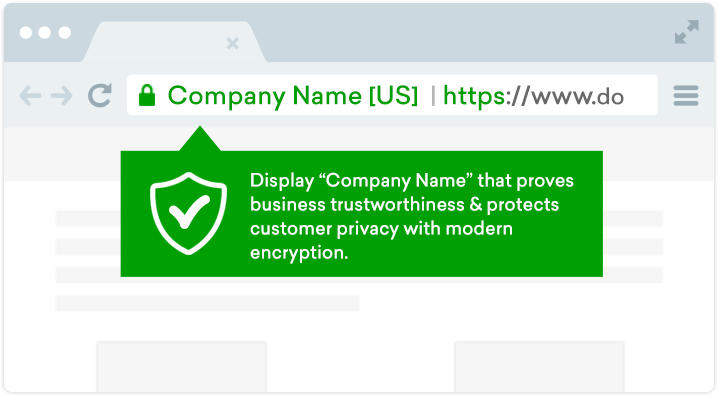
\includegraphics[width=11cm,height=6.5cm]{ev.png}
      \end{center}
      \caption{Validación extendida (Captura antigua)}
   \end{figure}
\end{center}

  \subsubsection*{Tipos de certificados}

  \paragraph*{Dominio Simple}
  Como sugiere el nombre, un certificado SSL de un solo dominio solo 
  se puede usar en un solo dominio o IP. Este se considera el tipo de 
  certificado SSL predeterminado. 
  
  \paragraph*{Multi-Dominio}
  Este tipo de SSL es un certificado para todos los usos. Permiten cifrar 
  hasta 250 dominios diferentes y subdominios 
  ilimitados. Desafortunadamente, no está disponible en EV.
  
  \paragraph*{Wildcard}
  
  Los \emph{wildcard} están diseñados específicamente para cifrar un dominio y 
  todos los subdominios que lo acompañan (también representado como *.dominio.com). 
  Desafortunadamente, los \emph{wildcard} solo están disponibles en los 
  niveles DV y OV.
  
  \paragraph*{Multi-Dominio Wildcard}
  Los \emph{wildcard} multidominio pueden cifrar hasta 250 dominios diferentes 
  y subdominios ilimitados. Desafortunadamente, no está disponible en EV.

  
\subsubsection*{Validación de propiedad de dominio}

Los certificados se utilizan con mayor frecuencia para autenticar 
nombres de dominio. Por lo tanto, se confía en las autoridades de 
certificación (CA) para verificar que un solicitante de un certificado 
represente legítimamente el nombre de dominio en el certificado.

Los diferentes tipos de certificados reflejan diferentes tipos de 
verificación de CA. Los certificados de “Validación de dominio” (DV) son 
el tipo más común. La única validación que debe realizar la CA en el 
proceso de emisión de un certificado DV es verificar que el solicitante 
tiene un control efectivo del dominio. La CA no está obligada a intentar 
verificar la identidad real del solicitante. Esto difiere en los certificados 
de “Validación de la organización” y “Validación extendida”, 
donde el proceso está destinado a verificar también la identidad real del 
solicitante.

ACME (\emph{Automatic Certificate Management Environment})
permite a un cliente 
la automatización de gestión de certificados 
mediante un conjunto de mensajes transmitidos a través de HTTPS. La 
emisión de certificados mediante el protocolo ACME se asemeja al proceso 
de emisión de una CA tradicional, en el que un usuario crea una cuenta, 
solicita un certificado y demuestra el control de los dominios con el 
certificado para que la CA emita el certificado solicitado.


ACME utiliza un \emph{framework} de desafío/respuesta extensible para la validación 
de dominios. El servidor envía al cliente un conjunto de desafíos, y el cliente 
responde enviando la respuesta al mismo en una solicitud POST a una URL de desafío.

Los diferentes desafíos permiten al servidor obtener pruebas de diferentes 
aspectos del control sobre un dominio. En los desafíos como HTTP y 
DNS, el cliente demuestra directamente su capacidad para hacer ciertas 
acciones relacionadas con el dominio. Es de gran utilidad explicar los 
diferentes tipos de desafíos que se puede ofrecer a un cliente, ya que uno 
es el mas común, sin embargo, al hablar de redes internas, no lo podremos 
utilizar, e iremos por la otra opción, un tanto menos conocida.


\paragraph*{Desafío HTTP}

Con la validación HTTP, el cliente prueba su control sobre un nombre de dominio al 
demostrar que puede guardar recursos HTTP en un servidor accesible bajo ese nombre 
de dominio. El servidor ACME desafía al cliente solicitándole un archivo en una ruta 
específica, con una cadena específica como contenido.

Este es el tipo de desafío más común en la actualidad. El servidor le da un token 
a su cliente ACME y su cliente ACME coloca un archivo en su servidor web 
en {http://\<SU\_DOMINIO\>/.well-known/acme-challenge/\<TOKEN\>}. Ese archivo contiene 
el token, más una huella digital de la clave de su cuenta.

Una vez que el cliente le dice al servidor que el archivo está listo, el servidor 
intenta recuperarlo. Al recibir una respuesta, el servidor construye y almacena la 
autorización de la clave a partir del valor del “token” de desafío y la clave de 
la cuenta del cliente actual.

Dado un par de desafío/respuesta, el servidor verifica el control del dominio por 
parte del cliente verificando que el recurso se aprovisionó como se esperaba.

Ventajas:
\begin{itemize}
   \setlength\itemsep{-0.6em}
   \item Es fácil de automatizar sin conocimientos adicionales sobre la configuración de un dominio.
   \item Funciona con servidores web estándar.
\end{itemize}

Desventajas:
\begin{itemize}
   \setlength\itemsep{-0.6em}
   \item No funciona si su ISP bloquea el puerto 80 (esto es raro, pero algunos ISP residenciales lo hacen).
   \item Let's Encrypt no le permite utilizar este desafío para emitir certificados Wildcard.
   \item Si tiene varios servidores web, debe asegurarse de que el archivo esté disponible en todos ellos.
\end{itemize}
   
Este desafío está fuera de nuestro alcance, ya que partimos de la premisa de que 
el tráfico que queremos proteger nunca saldrá a Internet, lo que implica que no 
tendremos ni puertos ni direcciones expuestas para que un servidor externo pueda 
verificar el recurso mencionado anteriormente. 


\paragraph*{Desafío DNS}
Cuando el identificador que se está validando es un nombre de dominio, el cliente 
puede demostrar el control de ese dominio proporcionando un registro DNS de tipo 
TXT que contenga un valor designado.

Un cliente cumple este desafío construyendo una clave de autorización a partir del 
valor de un token proporcionado y la clave de la cuenta del cliente. A continuación, el 
cliente calcula un hash SHA-256 de la clave de 
autorización.
El registro proporcionado al DNS contiene la codificación de URL base64 de este 
hash. 

\noindent Ejemplo:

Si se desea validar el nombre de dominio “www.ejemplo.org”, el cliente 
proporcionaría el siguiente registro DNS:

\begin{verbatim}
   _acme-challenge.www.ejemplo.org: "gfj9Xq...Rg85nM"
\end{verbatim}

Al recibir una respuesta, el servidor construye y almacena la llave de autorización
clave a partir del valor del “token” del desafío y la clave de la cuenta del cliente actual.

\noindent Para validar un desafío de DNS, el servidor realiza los siguientes pasos:

\begin{enumerate}
   \setlength\itemsep{-0.6em}
   \item Calcula el hash SHA-256 de la clave de autorización almacenada.
   \item Consulta los registros TXT para el nombre de dominio de validación.
   \item Verifica que el contenido de uno de los registros TXT coincida con el valor de hash.
\end{enumerate}

   
Si todas las verificaciones anteriores tienen éxito, entonces la validación es exitosa. 
Si no se encuentra ningún registro DNS, o si el registro DNS y el contenido del mismo 
no pasan estas comprobaciones, la validación falla.


\section{Protocolos asociados a la consulta de un sitio (DNS)}
    \subsection{¿Que es el protocolo DNS?} 







\chapter{Network Security Attacks: basic concepts} 
    \label{capDesc}
%-*- ES -*-
%----------------------------------------------------------------------
% Capitulo 7: Descripción del problema

En éste capítulo se verá por qué los protocolos http y smtp son inseguros, introducción al snnifin, spoofing, arp attack
%----------------------------------------------------------------------

(Agregar una intro)

\section{Establishing Authority}

HTTP relies on the notion of an authoritative response: a response
that has been determined by (or at the direction of) the authority
identified within the target URI to be the most appropriate response
for that request given the state of the target resource at the time
of response message origination.  Providing a response from a
non-authoritative source, such as a shared cache, is often useful to
improve performance and availability, but only to the extent that the
source can be trusted or the distrusted response can be safely used.

Unfortunately, establishing authority can be difficult.  For example,
phishing is an attack on the user's perception of authority, where
that perception can be misled by presenting similar branding in
hypertext, possibly aided by userinfo obfuscating the authority
component (see Section 2.7.1).  User agents can reduce the impact of
phishing attacks by enabling users to easily inspect a target URI
prior to making an action, by prominently distinguishing (or
rejecting) userinfo when present, and by not sending stored
credentials and cookies when the referring document is from an
unknown or untrusted source.

When a registered name is used in the authority component, the "http"
URI scheme (Section 2.7.1) relies on the user's local name resolution
service to determine where it can find authoritative responses.  This
means that any attack on a user's network host table, cached names,
or name resolution libraries becomes an avenue for attack on
establishing authority.  Likewise, the user's choice of server for
Domain Name Service (DNS), and the hierarchy of servers from which it
obtains resolution results, could impact the authenticity of address
mappings; DNS Security Extensions are one way to
improve authenticity.

Furthermore, after an IP address is obtained, establishing authority
for an "http" URI is vulnerable to attacks on Internet Protocol
routing.


\section{Risks of Intermediaries}

By their very nature, HTTP intermediaries are men-in-the-middle and,
thus, represent an opportunity for man-in-the-middle attacks.
Compromise of the systems on which the intermediaries run can result
in serious security and privacy problems.  Intermediaries might have
access to security-related information, personal information about
individual users and organizations, and proprietary information
belonging to users and content providers.  A compromised
intermediary, or an intermediary implemented or configured without
regard to security and privacy considerations, might be used in the
commission of a wide range of potential attacks.

Intermediaries that contain a shared cache are especially vulnerable
to cache poisoning attacks.
Implementers need to consider the privacy and security implications
of their design and coding decisions, and of the configuration
options they provide to operators (especially the default
configuration).

Users need to be aware that intermediaries are no more trustworthy
than the people who run them; HTTP itself cannot solve this problem.

\section{Attacks via Protocol Element Length}

Because HTTP uses mostly textual, character-delimited fields, parsers
are often vulnerable to attacks based on sending very long (or very
slow) streams of data, particularly where an implementation is
expecting a protocol element with no predefined length.



\section{Response Splitting}

Response splitting (a.k.a, CRLF injection) is a common technique,
used in various attacks on Web usage, that exploits the line-based
nature of HTTP message framing and the ordered association of
requests to responses on persistent connections [Klein].  This
technique can be particularly damaging when the requests pass through
a shared cache.

Response splitting exploits a vulnerability in servers (usually
within an application server) where an attacker can send encoded data
within some parameter of the request that is later decoded and echoed
within any of the response header fields of the response.  If the
decoded data is crafted to look like the response has ended and a
subsequent response has begun, the response has been split and the
content within the apparent second response is controlled by the
attacker.  The attacker can then make any other request on the same
persistent connection and trick the recipients (including
intermediaries) into believing that the second half of the split is
an authoritative answer to the second request.

For example, a parameter within the request-target might be read by
an application server and reused within a redirect, resulting in the
same parameter being echoed in the Location header field of the
response.  If the parameter is decoded by the application and not
properly encoded when placed in the response field, the attacker can
send encoded CRLF octets and other content that will make the
application's single response look like two or more responses.


\section{Request Smuggling}

Request smuggling ([Linhart]) is a technique that exploits
differences in protocol parsing among various recipients to hide
additional requests (which might otherwise be blocked or disabled by
policy) within an apparently harmless request.  Like response
splitting, request smuggling can lead to a variety of attacks on HTTP
usage.


\section{Message Integrity}

HTTP does not define a specific mechanism for ensuring message
integrity, instead relying on the error-detection ability of
underlying transport protocols and the use of length or
chunk-delimited framing to detect completeness.  Additional integrity
mechanisms, such as hash functions or digital signatures applied to
the content, can be selectively added to messages via extensible
metadata header fields.  Historically, the lack of a single integrity
mechanism has been justified by the informal nature of most HTTP
communication.  However, the prevalence of HTTP as an information
access mechanism has resulted in its increasing use within
environments where verification of message integrity is crucial.

User agents are encouraged to implement configurable means for
detecting and reporting failures of message integrity such that those
means can be enabled within environments for which integrity is
necessary.  For example, a browser being used to view medical history
or drug interaction information needs to indicate to the user when
such information is detected by the protocol to be incomplete,
expired, or corrupted during transfer.  Such mechanisms might be
selectively enabled via user agent extensions or the presence of
message integrity metadata in a response.  At a minimum, user agents
ought to provide some indication that allows a user to distinguish
between a complete and incomplete response message (Section 3.4) when
such verification is desired.

\section{Message Confidentiality}

HTTP relies on underlying transport protocols to provide message
confidentiality when that is desired.  HTTP has been specifically
designed to be independent of the transport protocol, such that it
can be used over many different forms of encrypted connection, with
the selection of such transports being identified by the choice of
URI scheme or within user agent configuration.

\section{Tipes of Attacks}
There are mainly two types of network attacks – passive attack and active attack

Passive: This type of attack happens when sensitive information is monitored and
analyzed, possibly compromising the security of enterprises and their customers.
In short, network intruder intercepts data traveling through the network.
• Active: This type of attack happens when information is modified, altered or
demolished entirely by a hacker. Here the interloper starts instructions to disturb
the network’s regular process.

So the motives behind passive attackers and active attackers are totally different.
Whereas the motive of passive attackers is simply to steal sensitive information and
to analyze the traffic to steal future messages, the motive of active attackers is to stop
normal communication between two legitimate entities.
\subsection{Passive Attacks}
Passive attackers aremainly interested in stealing sensitive information. This happens
without the knowledge of the victim. As such passive attacks are difficult to detect
and thereby secure the network. The following are some of the passive attacks that
are in existence [7].
\begin{itemize}
    \item Traffic Analysis: Attacker senses the communication path between the sender
    and receiver.
    \item Monitoring: Attacker can read the confidential data, but he cannot edit or modify
    the data.
    \item Eavesdropping: This type of attack occurs in the mobile ad-hoc network where
    basically the attacker finds out some secret or confidential information from
    communication.
\end{itemize}

\subsection{Active Attacks}
The active attacks happen in such a manner so as to notify the victims that their
systems have been compromised. As a result, the victim stops communication with
the other party. Some of the active attacks are as follows [8].
\begin{itemize}
    \item Modification: Some alterations in the routing route is performed by the malicious
    node. This results in causing the sender to send messages through the long route,
    which causes communication delay. This is an attack on integrity as shown in
    Fig. 2.
    \item Wormhole: This attack is also called a tunneling attack. A packet is received
    by an attacker at one point. He then tunnels it to another malicious node in the
    network. This causes a beginner to assume that he found the shortest path in the
    network as shown in Fig. 3.
    \item Fabrication: A malicious node generates a false routing message that causes the
    generation of incorrect information about the route between devices. This is an
    attack on authenticity as shown in Fig. 4.    
    \item Spoofing: A malicious node miss-present his identity so that the sender changes
    his topology as shown in Fig. 5.
    \item Denial of services: A malicious node sends a message to the node and consumes
    the bandwidth of the network as given in Fig.
    \item  Man-in-the-middle: Attack—Also called a hijacking attack, it is an attack where
    the attacker secretly alters and relays the communications between two legitimate
    parties without their knowledge. These parties in turn are unaware of the secret
    hacker consider that they are doing direct communication with each other [13].
    Figure 12 depicts this attack.
\end{itemize}

\section{Caso de estudio: Sniffing de la red para obtener credenciales}

\subsection{Herramienta Utilizadas} 
    

\subsubsection*{Kali Linux}
Kali Linux es una distribución de Linux (basada en Debian) centrada en la seguridad. 
Es una versión renombrada de la famosa distribución de Linux conocida como Backtrack, 
que venía con un enorme repositorio de herramientas de piratería de código abierto, 
para pruebas de penetración de aplicaciones \emph{web}, inalámbricas y de red. 

\begin{center}
    \begin{figure}   
       \begin{center}
          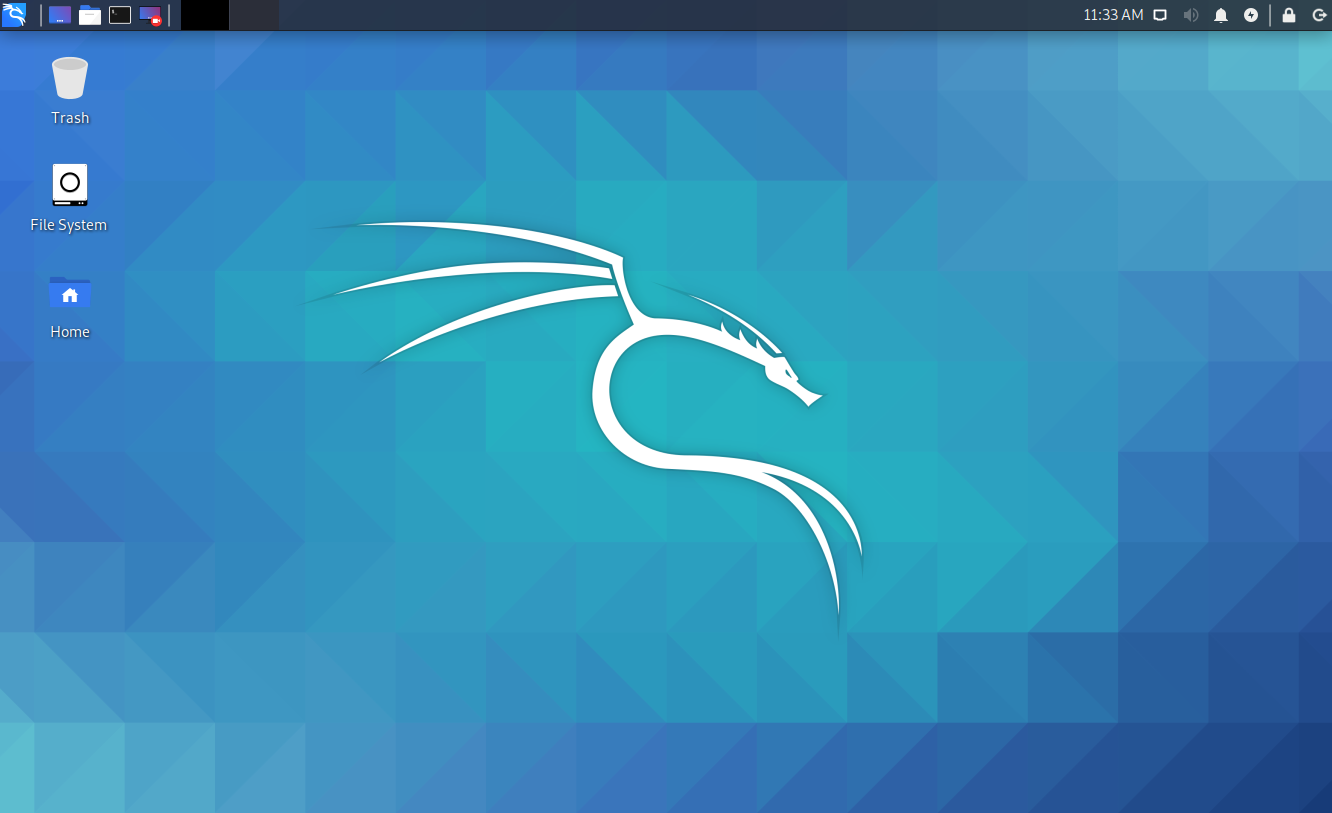
\includegraphics[width=11cm,height=7cm]{ataque-1.png}
       \end{center}
       \caption{Escritorio de Kali Linux}
    \end{figure}
 \end{center}
 

Kali Linux contiene muchas herramientas preinstaladas con 
todas las dependencias y ya está lista para usar. Esto nos permite tener que prestar 
más atención a las pruebas y no a la instalación de la herramienta. Las actualizaciones 
para las herramientas instaladas en Kali Linux se publican con mayor frecuencia, 
lo que le ayuda a mantener las a las mismas actualizadas.

Esta distribución contiene las herramientas necesarias para realizar nuestro
ataque.

\subsubsection*{Wireshark}
Wireshark es uno de los analizadores de protocolos de red más populares, es de 
código abierto y gratuito. Wireshark está preinstalado en Kali y es ideal para la 
resolución de problemas de red, análisis y, para este caso de estudio, una herramienta 
perfecta para monitorear el tráfico de posibles objetivos. Wireshark usa un kit de 
herramientas para implementar su interfaz de usuario y para capturar paquetes. 
Funciona de manera muy similar a un comando \emph{tcpdump}; sin embargo, nos brinda
una interfaz gráfica, posee opciones integradas de clasificación y filtrado.

\begin{center}
    \begin{figure}   
       \begin{center}
          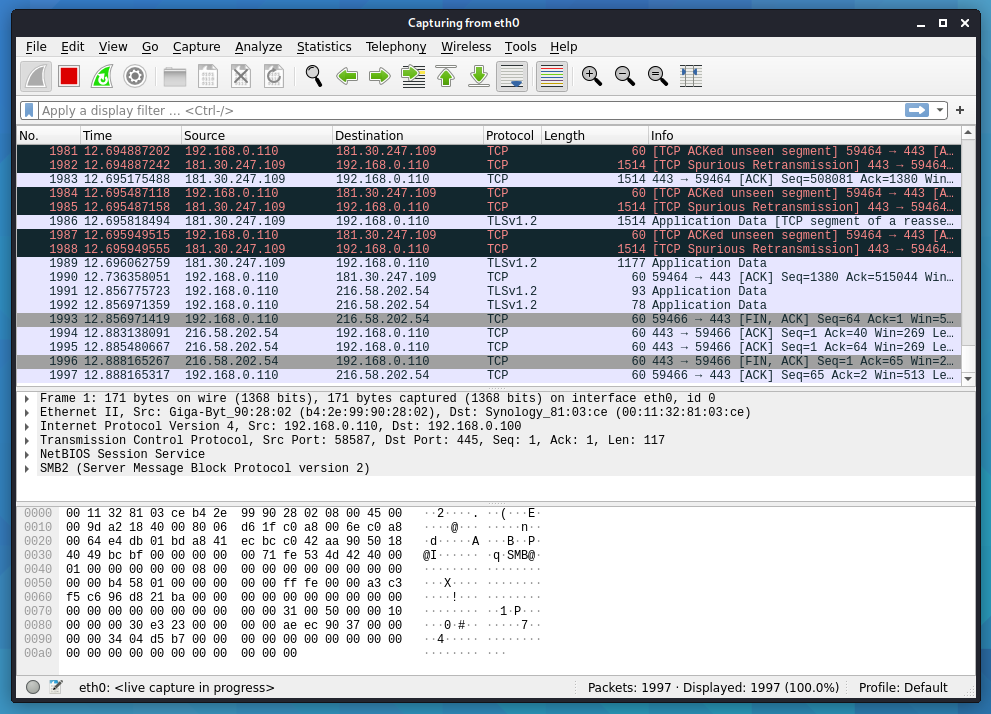
\includegraphics[width=10cm,height=7cm]{wireshark.png}
       \end{center}
       \caption{Interface del Wireshark}
    \end{figure}
 \end{center}
 
\subsubsection*{Ettercap}

\begin{center}
   \begin{figure}   
      \begin{center}
         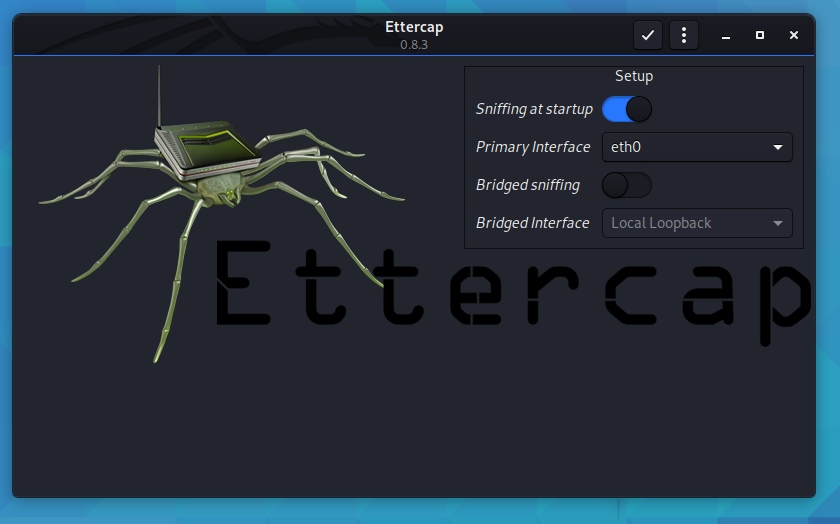
\includegraphics[width=10 cm,height=7cm]{ataque-2.png}
      \end{center}
      \caption{Ettercap}
   \end{figure}
\end{center}

Ettercap es un paquete completo gratuito y de código abierto para ataques basados 
en intermediarios. Ettercap se puede utilizar para análisis de protocolos de redes 
informáticas y auditorías de seguridad, con funciones de rastreo de conexiones en 
tiempo real y filtrado de contenido. Ettercap funciona configurando la interfaz de red 
del atacante en modo promiscuo y \emph{ARP} para envenenar las máquinas víctimas.



\subsection{Realización del ataque}

\begin{center}
    \begin{figure}   
       \begin{center}
          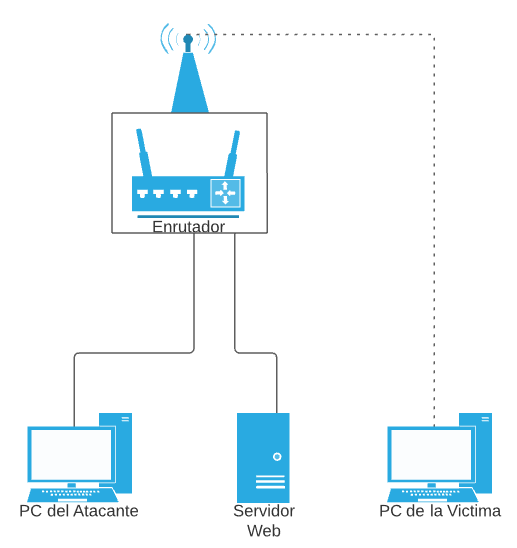
\includegraphics[width=9cm,height=9cm]{red.png}
       \end{center}
       \caption{Escenario montado}
    \end{figure}
 \end{center}

La idea principal de esta sección es demostrar que, encontrándose en una red interna
y con herramientas ya desarrolladas y libres, es posible realizar un ataque 
sin necesidad de conocer a fondo la implementación de la misma ni de tener mayores
privilegios.

El escenario consiste en crear una página web con un 
simple formulario donde se debe completar con usuario y contraseña, y un 
submit el cual envía esta información desde el cliente hasta el 
servidor web. El envío de este formulario contiene la información confidencial,
 por lo que en un escenario seguro ningún
intermediario podría obtener estos datos. Dado que este tráfico va a 
circular por HTTP, demostraremos como nos podemos hacer de las credenciales
ingresadas por el usuario.

\begin{center}
   \begin{figure}   
      \begin{center}
         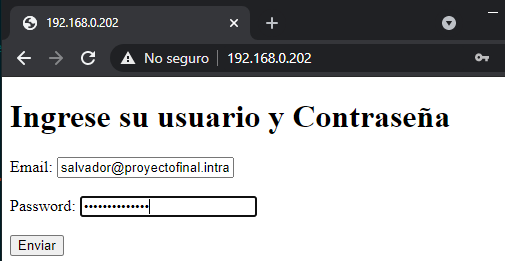
\includegraphics[width=10cm,height=6cm]{form.png}
      \end{center}
      \caption{Formulario montado}
   \end{figure}
\end{center}

Recordar que esto fue realizado en una red interna donde son todos equipos de nuestra propiedad.


\subsection{Preparando Ettercap para el ataque ARP Poisoning}

Lo primero que debemos hacer, en la lista de aplicaciones, es buscar el apartado 
\emph{Sniffing} y \emph{Spoofing}, ya que es allí donde encontraremos las herramientas necesarias
 para llevar a cabo este ataque. A continuación, abriremos Ettercap.

\begin{center}
    \begin{figure}   
       \begin{center}
          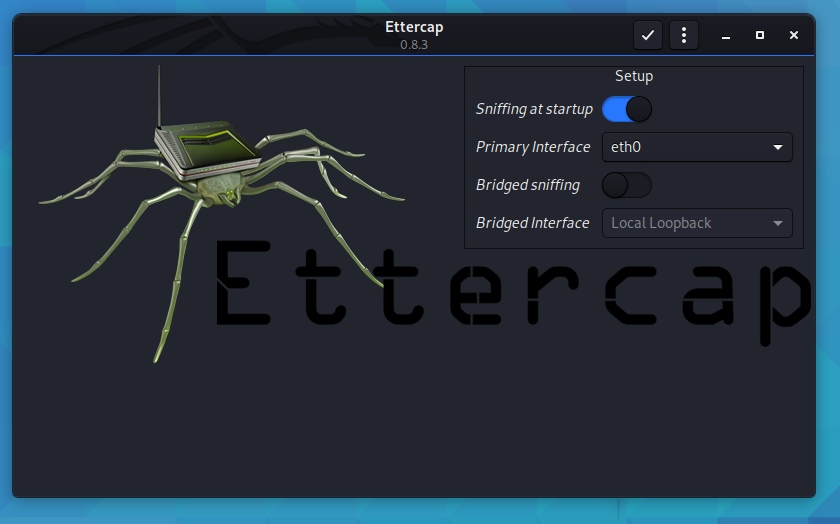
\includegraphics[width=9 cm,height=6cm]{ataque-2.png}
       \end{center}
       \caption{Ettercap}
    \end{figure}
 \end{center}

El siguiente paso es seleccionar la tarjeta de red con la que vamos a trabajar. Para 
ello, en el menú superior de Ettercap seleccionaremos Sniff $>$ Unified Sniffing y, 
cuando nos lo pregunte, seleccionaremos nuestra tarjeta de red (por ejemplo, en 
nuestro caso, eth0).

Luego se debe buscar todos los hosts conectados a nuestra red local. Para ello, 
seleccionaremos Hosts del menú de la parte superior y seleccionaremos la primera 
opción, Hosts List.

Allí deberían salirnos todos los hosts o dispositivos conectados a nuestra red. 
Sin embargo, en caso de que no salgan todos, podemos realizar una exploración 
completa de la red simplemente abriendo el menú Hosts y seleccionando la opción 
Scan for hosts. Tras unos segundos, la lista de antes se debería actualizar 
mostrando todos los dispositivos, con sus respectivas IPs y MACs, conectados 
a nuestra red.



\subsection{Nuestro Ettercap ya está listo. Ya podemos empezar con el ataque ARP Poisoning}

En caso de querer realizar un ataque dirigido contra un solo host, por ejemplo, 
suplantar la identidad de la puerta de enlace para monitorear las conexiones 
de la víctima, antes de empezar con el 
ataque debemos establecer los dos objetivos.

Para ello, debajo de la lista de hosts podemos ver tres botones, aunque nosotros 
prestaremos atención a los dos últimos:

    Target 1 – Seleccionamos la IP del dispositivo a monitorear, en este caso, 
    la computadora de la víctima, y pulsamos sobre dicho botón.

    Target 2 – Pulsamos la IP que queremos suplantar, en este caso, la de la 
    puerta de enlace y la del servidor web.

    \begin{center}
        \begin{figure}   
           \begin{center}
              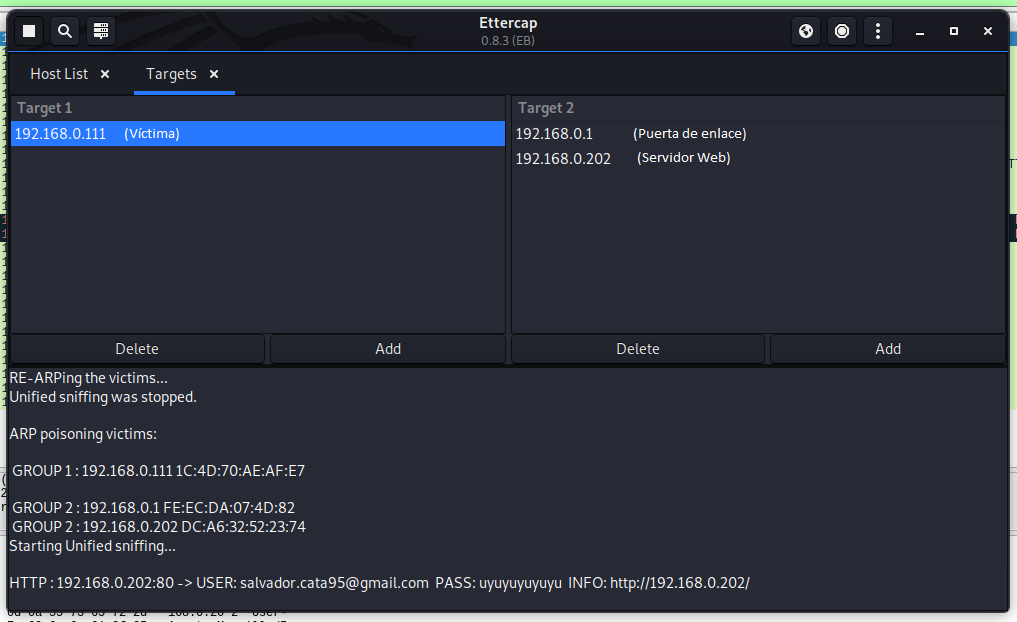
\includegraphics[width=17cm,height=9.5cm]{ataque-7-deta.png}
           \end{center}
           \caption{Ettercap}
        \end{figure}
     \end{center}

Todo listo. Ahora solo debemos elegir el menú MITM de la parte superior y, en él, 
escoger la opción ARP Poisoning. Nos aparecerá una pequeña ventana de configuración, 
en la cual debemos asegurarnos de marcar Sniff Remote Connections.
Pulsamos sobre Ok y el ataque dará lugar. Ahora ya podemos tener el control 
sobre el host que hayamos establecido como Target 1. Lo siguiente que debemos 
hacer es, ejecutar Wireshark para capturar todos los paquetes de 
red y analizarlos en busca de información interesante.

\begin{center}
   \begin{figure}   
      \begin{center}
         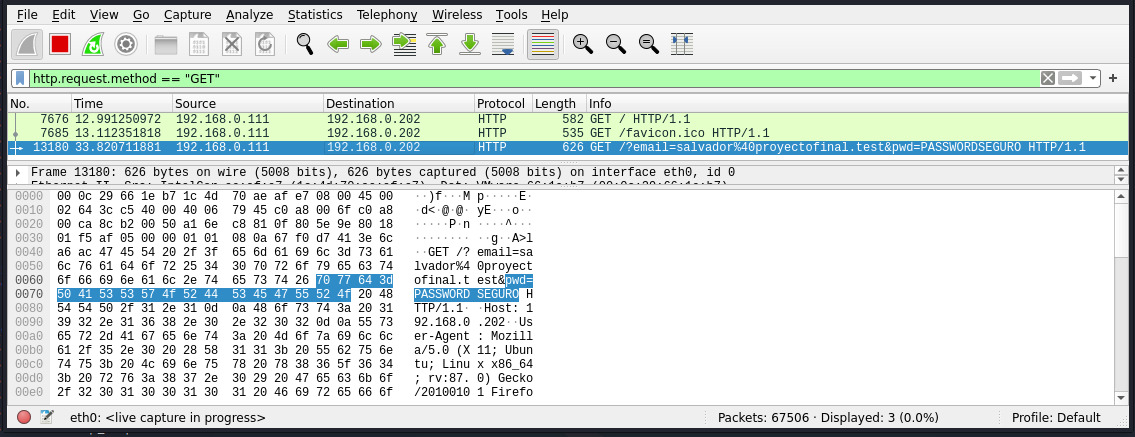
\includegraphics[width=17cm,height=7cm]{paquetes.png}
      \end{center}
      \caption{Paquetes capturados}
   \end{figure}
\end{center}

Como se puede ver, Wireshark nos permite filtrar el tráfico, y con el 
simple hecho de decirle que queremos mostrar los requerimientos GET
pudimos dar con el paquete que queríamos, en el request podemos ver
el usuario “salvador@proyectofinal.test” y la contraseña “PASSWORD SEGURO”




\chapter{Virtualización} \pagenumbering{arabic}
    \label{capVirtu}


Luego de haber explicado las debilidades del protocolo \emph{HTTP}, vamos a explorar las 
distintas soluciones encontradas, empezando con un pequeño marco teórico, el cual 
nos permitirá probar estas implementaciones y aplicarlas en un escenario de prueba.

La herramienta utilizada es \emph{Docker}, con ella es posible simular 
escenarios sin necesidad de tener cada uno de los servidores de manera física. Para
entenderlo un poco mejor, explicaremos lo que es la virtualización y profundizaremos 
en la virtualización basada en contenedores.
    
\section{Máquinas virtuales}

La virtualización brinda la capacidad de ejecutar aplicaciones, sistemas 
operativos o servicios del sistema en un entorno distinto. 
Obviamente, los mismos tienen que estar ejecutándose en un determinado 
sistema informático en un momento dado, pero la virtualización proporciona 
un nivel de abstracción lógica que libera las aplicaciones, los servicios 
del sistema e incluso el sistema operativo de estar vinculado a una 
pieza específica de \emph{hardware}. El enfoque de la virtualización hace 
que todo esto sea portátil a través de diferentes sistemas informáticos 
físicos.

El enfoque basado en \emph{VM} virtualiza el sistema operativo completo. Con esto nos referimos 
a la virtualización de discos, \emph{CPU} y \emph{NIC}. En otras palabras, podemos afirmar que se 
trata de virtualizar la arquitectura de conjunto de instrucciones completa, como ejemplo, 
la arquitectura \emph{x86}. 

\begin{center}
    \begin{figure}   
       \begin{center}
          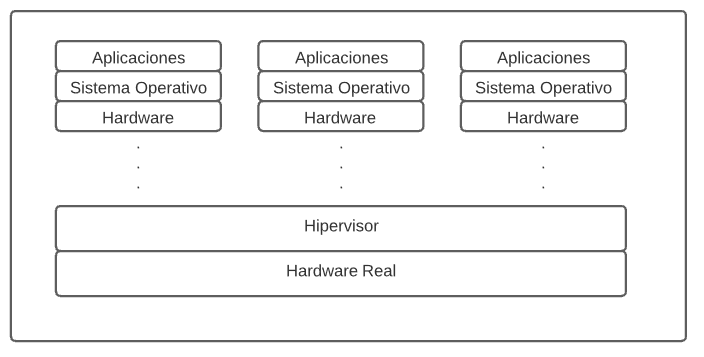
\includegraphics[width=12cm,height=7cm]{vm.png}
       \end{center}
       \caption{Virtualización}
    \end{figure}
 \end{center}

Para virtualizar un sistema operativo, se utiliza un \emph{software} especial, denominado
\emph{hipervisor}, y es el encargado, entre otras cosas, de aislar el sistema 
operativo de las máquinas virtuales y 
permitir crearlas y gestionarlas.

Una \emph{VM} debe satisfacer tres propiedades:
\begin{itemize}
    \setlength\itemsep{-0.6em}
    \item Aislamiento: debe aislar a los invitados entre sí. 
    \item Equivalencia: debe comportarse igual, con o sin virtualización. Esto 
    significa que se deben ejecutar la mayoría de las instrucciones en el \emph{hardware} 
    físico sin ninguna traducción hacia el \emph{hardware} virtual.
    \item Rendimiento: Debería funcionar tan bien como lo hace sin ninguna 
    virtualización. Esto nuevamente significa que la sobrecarga de ejecutar 
    una VM debe ser mínima.
\end{itemize}

\section{Virtualización basada en Contenedores}

Esta forma de virtualización no abstrae el \emph{hardware}, sino que utiliza técnicas 
dentro del \emph{kernel} de Linux para aislar las rutas de acceso para diferentes recursos. 
Establece un límite lógico dentro del mismo sistema operativo. Como resultado, obtenemos 
un sistema de archivos raíz separado, un árbol de procesos separado, un subsistema 
de red separado, etc.

\begin{center}
    \begin{figure}   
       \begin{center}
          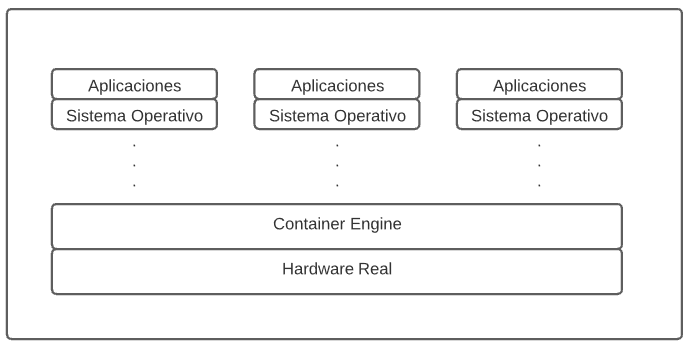
\includegraphics[width=12cm,height=7cm]{contenedores.png}
       \end{center}
       \caption{Virtualización basada en Contenedores}
    \end{figure}
 \end{center}

El \emph{kernel} de Linux se compone de varios componentes y funcionalidades; los relacionados 
con contenedores son los siguientes:
\begin{itemize}
    \setlength\itemsep{-0.6em}
    \item Grupos de control (\emph{Cgroups})
    \item Espacios de nombres (Namespaces)
    \item Linux con seguridad mejorada (SELinux)
\end{itemize}

\subsection*{Cgroups}
La funcionalidad de \emph{cgroup} permite limitar y priorizar recursos, como \emph{CPU}, RAM, 
la red, el sistema de archivos, etc. El objetivo principal es no exceder los 
recursos, para evitar desperdiciar recursos que podrían ser necesarios para 
otros procesos.

\subsection*{Espacios de nombres}
La funcionalidad del espacio de nombres permite particionar los recursos del kernel, 
de modo que un conjunto de procesos ve un conjunto de recursos, mientras que otro 
conjunto de procesos ve un conjunto diferente de recursos. La característica funciona 
al tener el mismo espacio de nombres para estos recursos en los distintos conjuntos 
de procesos, pero esos nombres se refieren a recursos distintos. Algunos nombres 
de recursos que pueden existir en varios espacios son los ID de proceso, nombres 
de host, ID de usuario, nombres de archivo y algunos nombres asociados con el 
acceso a la red y la comunicación entre procesos. 

Cuando se inicia un sistema 
Linux, solo se crea un espacio de nombres. Los procesos y recursos se unirán 
al mismo espacio de nombres, hasta que se cree un espacio de nombres diferente, 
se le asignen recursos y los procesos se unan a él.

\subsection*{SELinux}
SELinux es un módulo del \emph{kernel} de Linux que proporciona un mecanismo para hacer 
cumplir la seguridad del sistema, con políticas específicas. Básicamente, SELinux 
puede limitar el acceso de los programas a archivos y recursos de red. La idea es 
limitar los privilegios de los programas y demonios al mínimo, de modo que pueda 
limitar el riesgo de que el sistema se detenga.

Lo contenedores utilizan los recursos directamente y no necesitan de un emulador en 
absoluto, cuantos menos recursos, mayor eficiencia. Se pueden ejecutar diferentes 
aplicaciones en el mismo host: aisladas a nivel de \emph{kernel} y aisladas por 
espacios de nombres y \emph{cgroups}. El \emph{kernel}, es decir, el Sistema Operativo,
 lo comparten todos los contenedores.

\subsection*{Contenedores}
Cuando hablamos de contenedores, nos referimos indirectamente a dos conceptos 
principales: una imagen de contenedor y una imagen de contenedor en ejecución. 
Una imagen de contenedor es la definición del contenedor, en donde el \emph{software} 
restante se instala como capas adicionales, como se muestra en el diagrama.

\begin{center}
    \begin{figure}   
       \begin{center}
          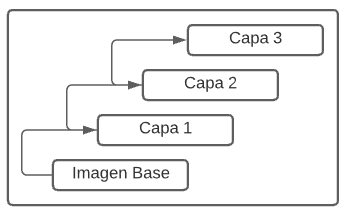
\includegraphics[width=7.5cm,height=5cm]{contenedores-capas.png}
       \end{center}
       \caption{Capas de contenedores}
       \label{capasContenedores}
    \end{figure}
 \end{center}

Una imagen de contenedor suele estar formada por varias capas (figura \ref{capasContenedores}).
La primera capa está dada por la imagen base, que proporciona las funcionalidades 
centrales del sistema operativo, con todas las herramientas necesarias para comenzar. 
Los equipos de desarrolladores a menudo trabajan construyendo sus propias capas sobre 
estas imágenes base. Los usuarios también pueden crear imágenes de aplicaciones más 
avanzadas, que no solo tienen un sistema operativo, sino que también incluyen 
herramientas de depuración y bibliotecas.

Los contenedores brindan aislamiento al aprovechar las tecnologías del \emph{kernel}, como 
\emph{cgroups}, espacios de nombres del \emph{kernel} y SELinux. Dado que  
utilizan un \emph{kernel} compartido y un host de contenedor, se reduce la cantidad de 
recursos necesarios para el contenedor en sí y son más livianos en comparación 
con las máquinas virtuales. 

Por lo mencionado anteriormente, podemos afirmar que los contenedores brindan una agilidad 
que no es factible con las \emph{VM}, y una prueba de esto es que solo se 
necesitan unos segundos para iniciar un nuevo contenedor. 
Además, los mismos admiten un 
modelo más flexible en lo que respecta a la utilización de la \emph{CPU} y los recursos 
de memoria, y permiten modos de ráfaga de recursos, donde las aplicaciones 
pueden consumir más recursos cuando es requerido, dentro de los límites definidos.


\section{\emph{Docker}}

\emph{Docker} es una herramienta de código abierto que automatiza la implementación de aplicaciones 
en contenedores. Fue escrito por el equipo de \emph{Docker} y publicado por ellos bajo la 
licencia Apache 2.0. Está diseñado para proporcionar 
un entorno ligero y rápido para implementar escenarios determinados, así como un flujo de 
trabajo 
eficiente para llevar ese código desde una computadora portátil a su entorno de prueba 
y luego a producción. De hecho, se puede comenzar con \emph{Docker} en un host mínimo que 
no ejecute nada más que un \emph{kernel} de Linux compatible y un binario de \emph{Docker}.



\subsection{Imágenes}
Las imágenes son los componentes básicos del mundo de \emph{Docker}. El uso común es 
lanzando los contenedores a partir de imágenes. Tienen un formato en capas, que 
se forman paso a paso utilizando una serie de instrucciones.

Se puede considerar a las imágenes como el “código fuente” de los contenedores. 
Son muy portátiles y se pueden compartir, almacenar y actualizar. .

\subsection{Registros}
\emph{Docker} almacena las imágenes que se crean en registros. Hay dos tipos de 
registros: públicos y privados. La herramienta opera el registro público de imágenes, 
llamado \emph{Docker} Hub. Se puede crear una cuenta y usarla para 
compartir y almacenar nuestras propias imágenes. También es posible almacenar 
las imágenes que desee y mantenerlas privadas en \emph{Docker} Hub. Estas imágenes 
pueden incluir código fuente u otra información de propiedad que se quiera 
mantener segura o solo compartir con otros miembros de su equipo u organización.

\subsection{Contenedores}
El \emph{software} permite construir e implementar contenedores dentro de los cuales se puede 
empaquetar aplicaciones y servicios. Como acabamos de mencionar, los contenedores 
se lanzan a partir de imágenes y estos pueden contener uno o más procesos en ejecución.

\noindent Un contenedor es:
\begin{itemize}
    \setlength\itemsep{-0.6em}
    \item Un formato de imagen.
    \item Un conjunto de operaciones estándar.
    \item Un entorno de ejecución.
\end{itemize}

Se puede hacer una analogía entre los contenedores de \emph{Docker} y los contenedores 
de envío estándar, utilizado para transportar mercancías a nivel mundial. 
En lugar de enviar mercancías, los contenedores de \emph{Docker} envían \emph{software}. 
Cada contenedor contiene una imagen de \emph{software}, su “carga”, y, al igual 
que su contraparte física, permite realizar un conjunto de operaciones. 
Por ejemplo, se puede crear, iniciar, detener, reiniciar y destruir. Como 
un contenedor de envío, \emph{Docker} no se preocupa por el contenido del contenedor 
cuando realiza estas acciones; por ejemplo, si un contenedor es un servidor \emph{web}, 
una base de datos o un servidor de aplicaciones. Cada contenedor se carga 
igual que cualquier otro. A \emph{Docker} tampoco le importa dónde envía su contenedor: 
se puede compilar en una computadora portátil, cargarlo en un registro, luego 
descargarlo en un servidor físico o virtual, probarlo, implementarlo en un 
clúster de una docena de \emph{hosts} y ejecutarlo. 




\chapter{Herramienta Utilizadas} 
    \label{capTools}

\subsubsection*{Kali Linux}
Kali Linux es una distribución de Linux (basada en Debian) centrada en la seguridad. 
Es una versión renombrada de la famosa distribución de Linux conocida como Backtrack, 
que venía con un enorme repositorio de herramientas de piratería de código abierto, 
para pruebas de penetración de aplicaciones \emph{web}, inalámbricas y de red. 

\begin{center}
    \begin{figure}   
       \begin{center}
          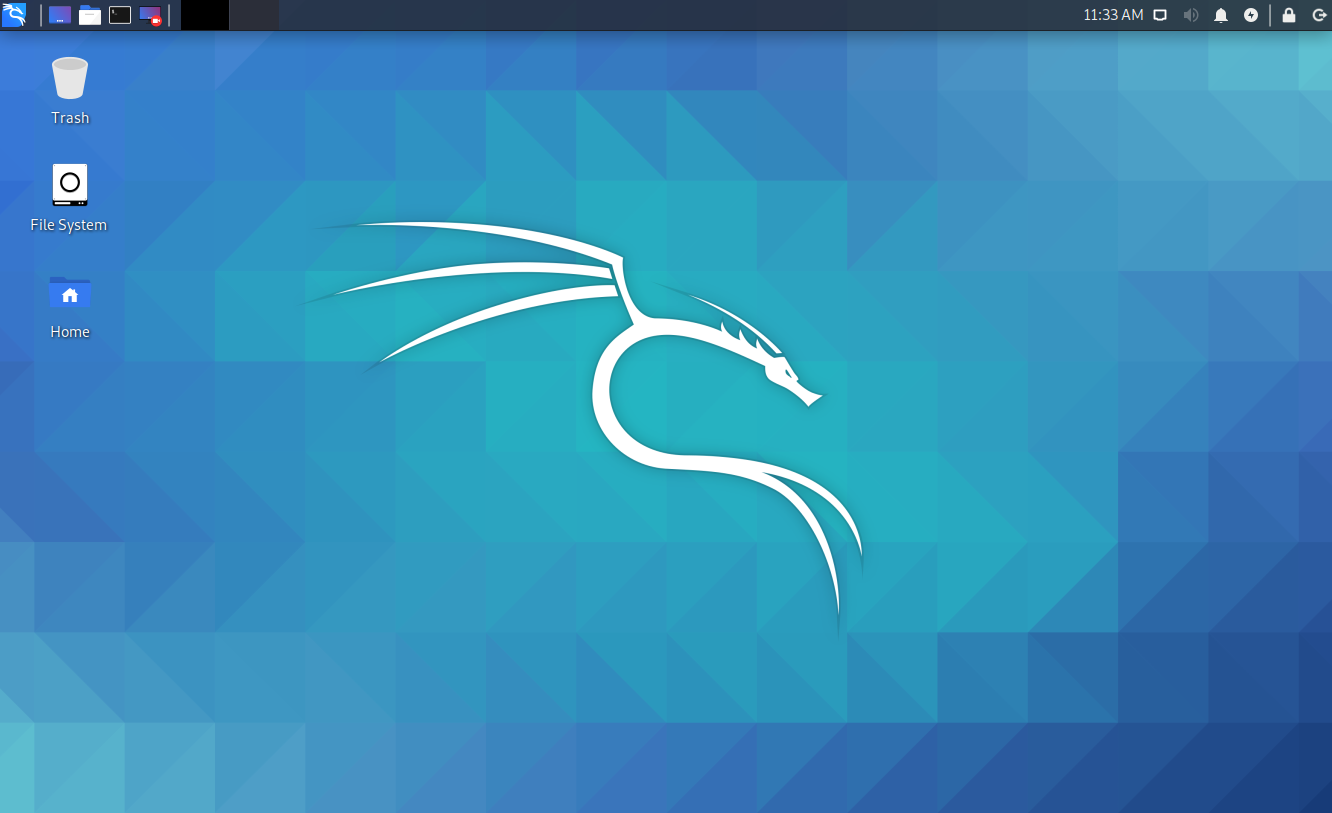
\includegraphics[width=11cm,height=7cm]{ataque-1.png}
       \end{center}
       \caption{Escritorio de Kali Linux}
    \end{figure}
 \end{center}
 

Kali Linux contiene muchas herramientas preinstaladas con 
todas las dependencias y ya está lista para usar. Esto nos permite tener que prestar 
más atención a las pruebas y no a la instalación de la herramienta. Las actualizaciones 
para las herramientas instaladas en Kali Linux se publican con mayor frecuencia, 
lo que le ayuda a mantener las a las mismas actualizadas.

Esta distribución contiene las herramientas necesarias para realizar nuestro
ataque.

\subsubsection*{Wireshark}
Wireshark es uno de los analizadores de protocolos de red más populares, es de 
código abierto y gratuito. Wireshark está preinstalado en Kali y es ideal para la 
resolución de problemas de red, análisis y, para este caso de estudio, una herramienta 
perfecta para monitorear el tráfico de posibles objetivos. Wireshark usa un kit de 
herramientas para implementar su interfaz de usuario y para capturar paquetes. 
Funciona de manera muy similar a un comando \emph{tcpdump}; sin embargo, nos brinda
una interfaz gráfica, posee opciones integradas de clasificación y filtrado.

\begin{center}
    \begin{figure}   
       \begin{center}
          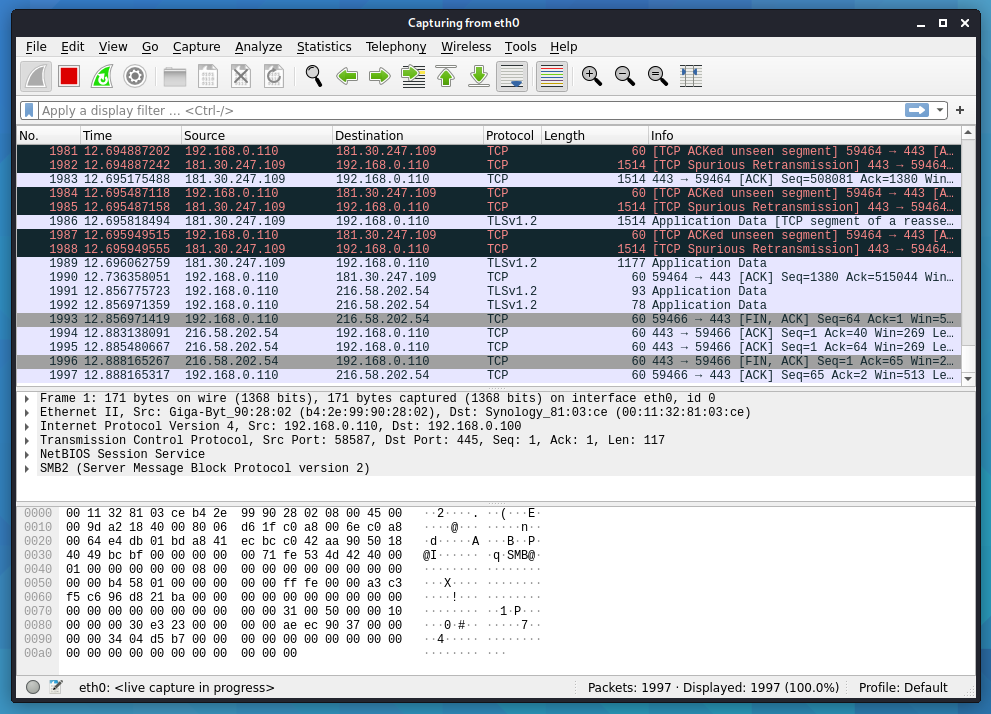
\includegraphics[width=10cm,height=7cm]{wireshark.png}
       \end{center}
       \caption{Interface del Wireshark}
    \end{figure}
 \end{center}
 
\subsubsection*{Ettercap}

\begin{center}
   \begin{figure}   
      \begin{center}
         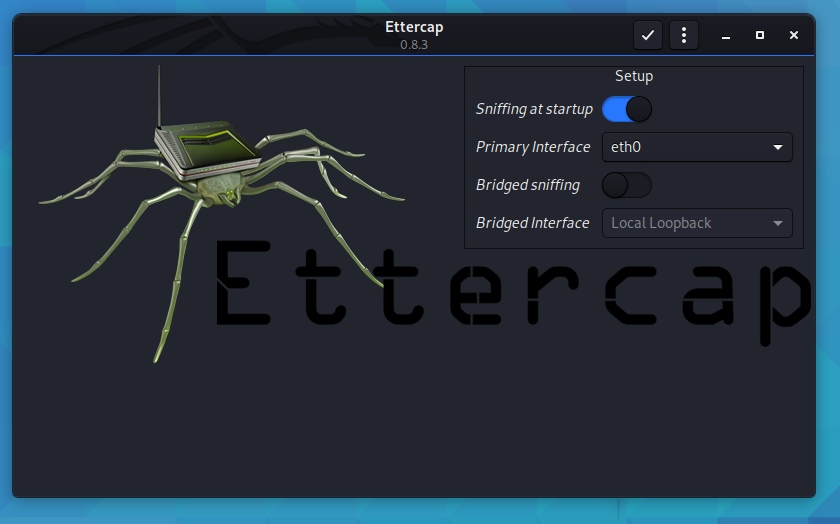
\includegraphics[width=10 cm,height=7cm]{ataque-2.png}
      \end{center}
      \caption{Ettercap}
   \end{figure}
\end{center}

Ettercap es un paquete completo gratuito y de código abierto para ataques basados 
en intermediarios. Ettercap se puede utilizar para análisis de protocolos de redes 
informáticas y auditorías de seguridad, con funciones de rastreo de conexiones en 
tiempo real y filtrado de contenido. Ettercap funciona configurando la interfaz de red 
del atacante en modo promiscuo y \emph{ARP} para envenenar las máquinas víctimas.



\chapter{Caso de estudio: Sniffing de la red para obtener credenciales } 
    \label{capCaseOfStudy}

\subsection{Herramienta Utilizadas} 
    

\subsubsection*{Kali Linux}
Kali Linux es una distribución de Linux (basada en Debian) centrada en la seguridad. 
Es una versión renombrada de la famosa distribución de Linux conocida como Backtrack, 
que venía con un enorme repositorio de herramientas de piratería de código abierto, 
para pruebas de penetración de aplicaciones \emph{web}, inalámbricas y de red. 

\begin{center}
    \begin{figure}   
       \begin{center}
          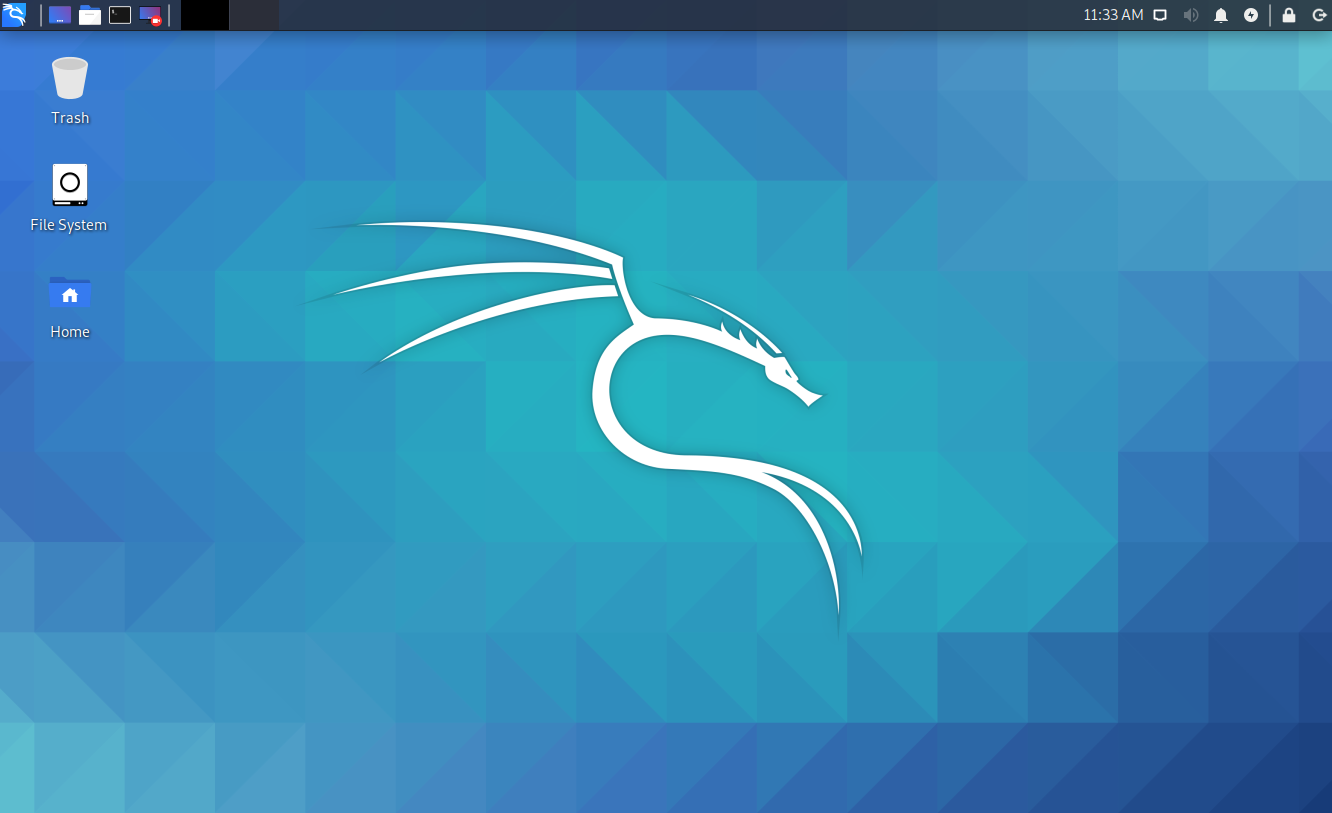
\includegraphics[width=11cm,height=7cm]{ataque-1.png}
       \end{center}
       \caption{Escritorio de Kali Linux}
    \end{figure}
 \end{center}
 

Kali Linux contiene muchas herramientas preinstaladas con 
todas las dependencias y ya está lista para usar. Esto nos permite tener que prestar 
más atención a las pruebas y no a la instalación de la herramienta. Las actualizaciones 
para las herramientas instaladas en Kali Linux se publican con mayor frecuencia, 
lo que le ayuda a mantener las a las mismas actualizadas.

Esta distribución contiene las herramientas necesarias para realizar nuestro
ataque.

\subsubsection*{Wireshark}
Wireshark es uno de los analizadores de protocolos de red más populares, es de 
código abierto y gratuito. Wireshark está preinstalado en Kali y es ideal para la 
resolución de problemas de red, análisis y, para este caso de estudio, una herramienta 
perfecta para monitorear el tráfico de posibles objetivos. Wireshark usa un kit de 
herramientas para implementar su interfaz de usuario y para capturar paquetes. 
Funciona de manera muy similar a un comando \emph{tcpdump}; sin embargo, nos brinda
una interfaz gráfica, posee opciones integradas de clasificación y filtrado.

\begin{center}
    \begin{figure}   
       \begin{center}
          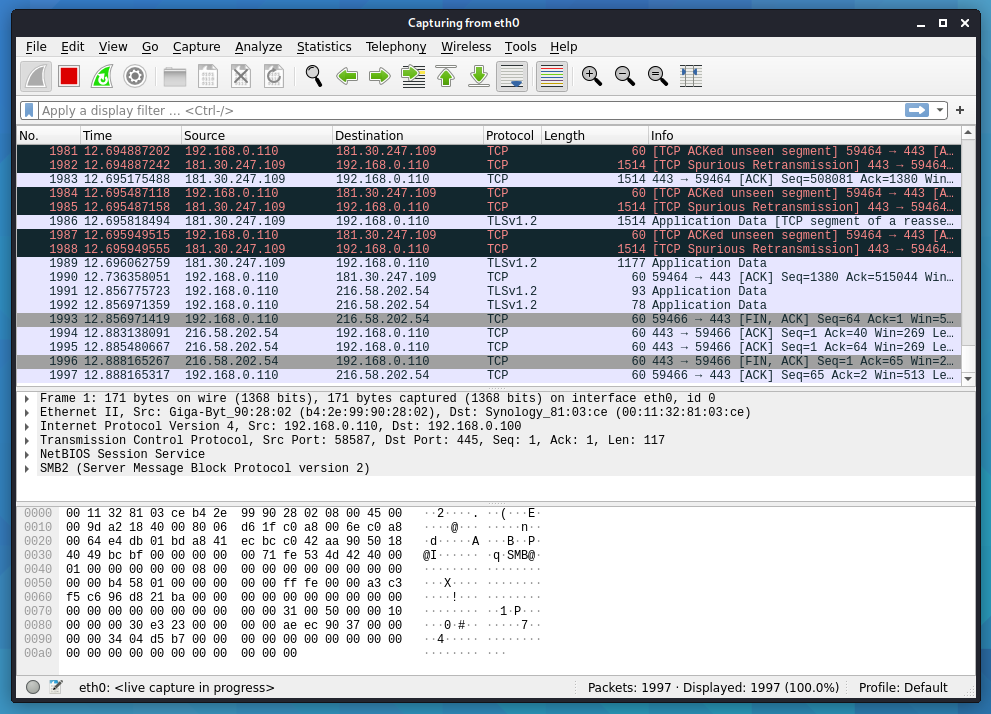
\includegraphics[width=10cm,height=7cm]{wireshark.png}
       \end{center}
       \caption{Interface del Wireshark}
    \end{figure}
 \end{center}
 
\subsubsection*{Ettercap}

\begin{center}
   \begin{figure}   
      \begin{center}
         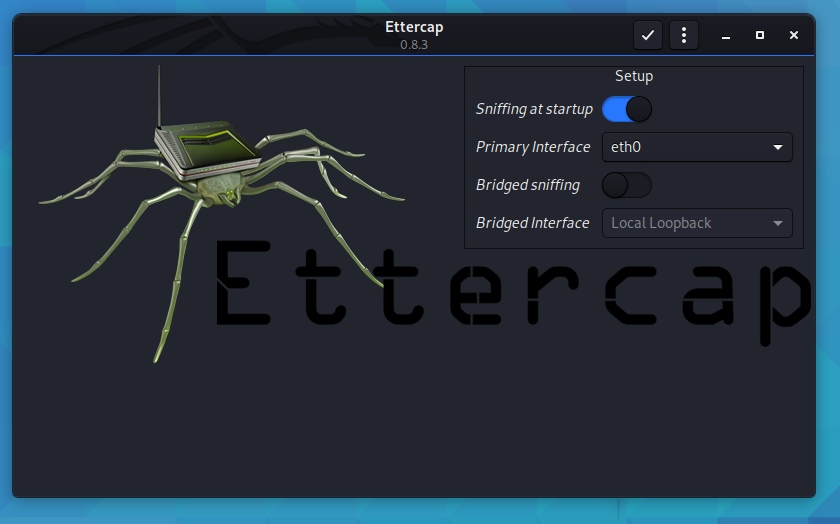
\includegraphics[width=10 cm,height=7cm]{ataque-2.png}
      \end{center}
      \caption{Ettercap}
   \end{figure}
\end{center}

Ettercap es un paquete completo gratuito y de código abierto para ataques basados 
en intermediarios. Ettercap se puede utilizar para análisis de protocolos de redes 
informáticas y auditorías de seguridad, con funciones de rastreo de conexiones en 
tiempo real y filtrado de contenido. Ettercap funciona configurando la interfaz de red 
del atacante en modo promiscuo y \emph{ARP} para envenenar las máquinas víctimas.



\subsection{Realización del ataque}

\begin{center}
    \begin{figure}   
       \begin{center}
          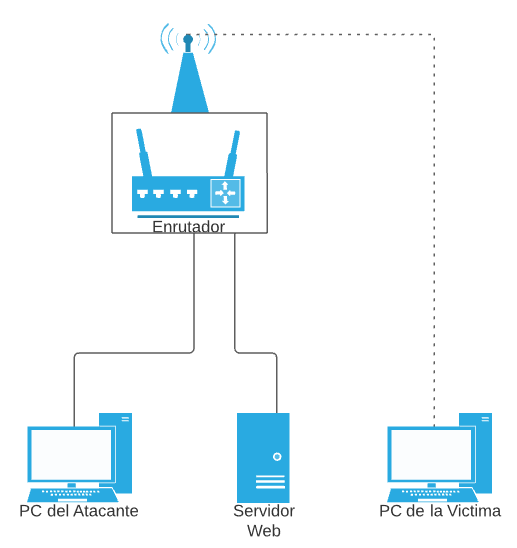
\includegraphics[width=9cm,height=9cm]{red.png}
       \end{center}
       \caption{Escenario montado}
    \end{figure}
 \end{center}

La idea principal de esta sección es demostrar que, encontrándose en una red interna
y con herramientas ya desarrolladas y libres, es posible realizar un ataque 
sin necesidad de conocer a fondo la implementación de la misma ni de tener mayores
privilegios.

El escenario consiste en crear una página web con un 
simple formulario donde se debe completar con usuario y contraseña, y un 
submit el cual envía esta información desde el cliente hasta el 
servidor web. El envío de este formulario contiene la información confidencial,
 por lo que en un escenario seguro ningún
intermediario podría obtener estos datos. Dado que este tráfico va a 
circular por HTTP, demostraremos como nos podemos hacer de las credenciales
ingresadas por el usuario.

\begin{center}
   \begin{figure}   
      \begin{center}
         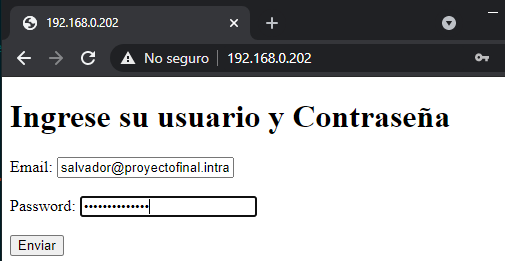
\includegraphics[width=10cm,height=6cm]{form.png}
      \end{center}
      \caption{Formulario montado}
   \end{figure}
\end{center}

Recordar que esto fue realizado en una red interna donde son todos equipos de nuestra propiedad.


\subsection{Preparando Ettercap para el ataque ARP Poisoning}

Lo primero que debemos hacer, en la lista de aplicaciones, es buscar el apartado 
\emph{Sniffing} y \emph{Spoofing}, ya que es allí donde encontraremos las herramientas necesarias
 para llevar a cabo este ataque. A continuación, abriremos Ettercap.

\begin{center}
    \begin{figure}   
       \begin{center}
          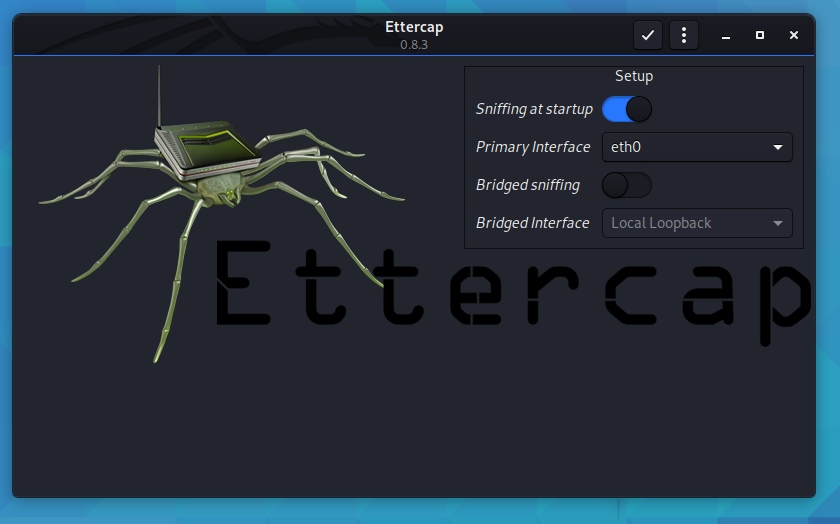
\includegraphics[width=9 cm,height=6cm]{ataque-2.png}
       \end{center}
       \caption{Ettercap}
    \end{figure}
 \end{center}

El siguiente paso es seleccionar la tarjeta de red con la que vamos a trabajar. Para 
ello, en el menú superior de Ettercap seleccionaremos Sniff $>$ Unified Sniffing y, 
cuando nos lo pregunte, seleccionaremos nuestra tarjeta de red (por ejemplo, en 
nuestro caso, eth0).

Luego se debe buscar todos los hosts conectados a nuestra red local. Para ello, 
seleccionaremos Hosts del menú de la parte superior y seleccionaremos la primera 
opción, Hosts List.

Allí deberían salirnos todos los hosts o dispositivos conectados a nuestra red. 
Sin embargo, en caso de que no salgan todos, podemos realizar una exploración 
completa de la red simplemente abriendo el menú Hosts y seleccionando la opción 
Scan for hosts. Tras unos segundos, la lista de antes se debería actualizar 
mostrando todos los dispositivos, con sus respectivas IPs y MACs, conectados 
a nuestra red.



\subsection{Nuestro Ettercap ya está listo. Ya podemos empezar con el ataque ARP Poisoning}

En caso de querer realizar un ataque dirigido contra un solo host, por ejemplo, 
suplantar la identidad de la puerta de enlace para monitorear las conexiones 
de la víctima, antes de empezar con el 
ataque debemos establecer los dos objetivos.

Para ello, debajo de la lista de hosts podemos ver tres botones, aunque nosotros 
prestaremos atención a los dos últimos:

    Target 1 – Seleccionamos la IP del dispositivo a monitorear, en este caso, 
    la computadora de la víctima, y pulsamos sobre dicho botón.

    Target 2 – Pulsamos la IP que queremos suplantar, en este caso, la de la 
    puerta de enlace y la del servidor web.

    \begin{center}
        \begin{figure}   
           \begin{center}
              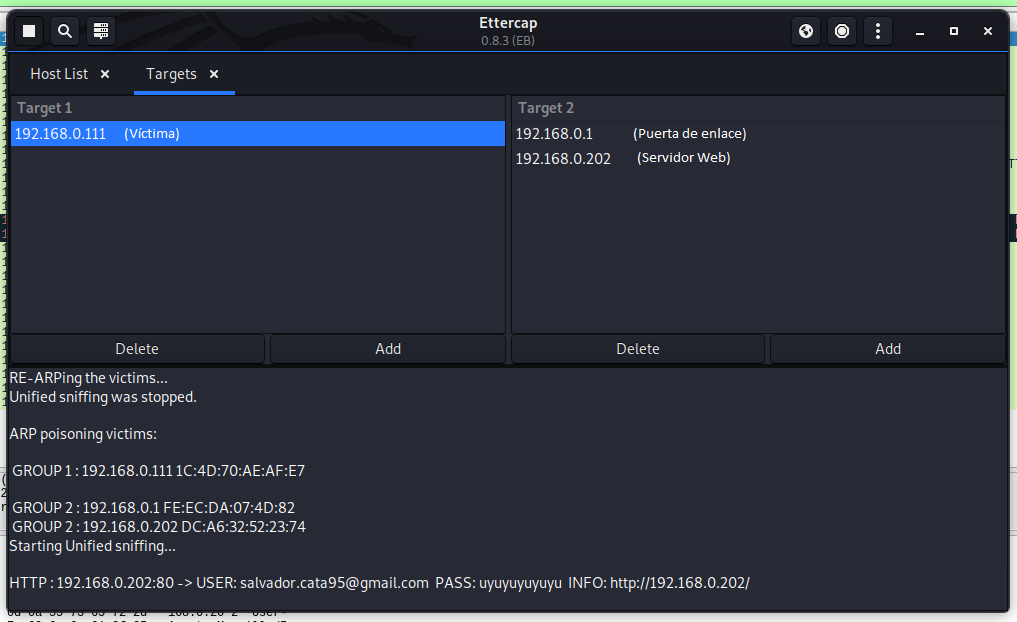
\includegraphics[width=17cm,height=9.5cm]{ataque-7-deta.png}
           \end{center}
           \caption{Ettercap}
        \end{figure}
     \end{center}

Todo listo. Ahora solo debemos elegir el menú MITM de la parte superior y, en él, 
escoger la opción ARP Poisoning. Nos aparecerá una pequeña ventana de configuración, 
en la cual debemos asegurarnos de marcar Sniff Remote Connections.
Pulsamos sobre Ok y el ataque dará lugar. Ahora ya podemos tener el control 
sobre el host que hayamos establecido como Target 1. Lo siguiente que debemos 
hacer es, ejecutar Wireshark para capturar todos los paquetes de 
red y analizarlos en busca de información interesante.

\begin{center}
   \begin{figure}   
      \begin{center}
         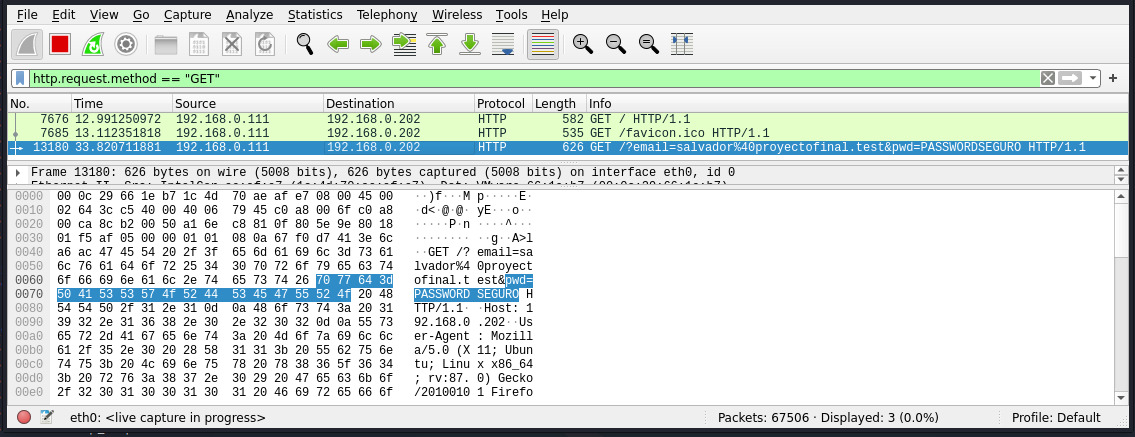
\includegraphics[width=17cm,height=7cm]{paquetes.png}
      \end{center}
      \caption{Paquetes capturados}
   \end{figure}
\end{center}

Como se puede ver, Wireshark nos permite filtrar el tráfico, y con el 
simple hecho de decirle que queremos mostrar los requerimientos GET
pudimos dar con el paquete que queríamos, en el request podemos ver
el usuario “salvador@proyectofinal.test” y la contraseña “PASSWORD SEGURO”




\chapter{Mejorando la seguridad en la navegación} 
    \label{capImp}

%-*- ES -*-
%----------------------------------------------------------------------
% Capitulo: Implementacion de la solución propuesta
%----------------------------------------------------------------------

\section{Propuestas: Introducción}

Se han investigado tres alternativas enfocadas en redes internas para mejorar la seguridad de las 
mismas, luego de eso se eligió la que más ventajas nos ofreció.
Las alternativas son las siguientes: Los certificados auto-firmados (\emph{Self-signed Certificates}), implementar
una entidad certificante interna, y la utilización de un certificado emitido por una entidad
certificante conocida.

\section{Propuesta 1: Self-signed Certificates}
Los certificados autofirmados son los menos útiles de los tres. Firefox facilita su uso 
de forma segura; crea una excepción en la primera visita, después de lo cual el 
certificado autofirmado se considera válido en las conexiones posteriores. Otros 
navegadores hacen que haga clic en una advertencia de certificado cada vez. A menos 
que esté comprobando la huella digital del certificado cada vez, no es posible hacer 
que ese certificado autofirmado sea seguro. Incluso con Firefox, puede resultar 
difícil utilizar estos certificados de forma segura.

\begin{center}
   \begin{figure}   
      \begin{center}
         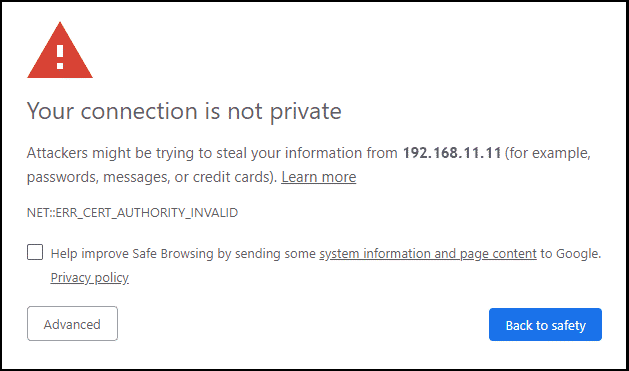
\includegraphics[width=13cm,height=9cm]{self-signed.png}
      \end{center}
      \caption{Advertencia Certificado Autofirmado}
   \end{figure}
\end{center}

Por ejemplo, para solicitar un certificado SSL de una CA de confianza como Verisign o 
GoDaddy, se debe enviar una Solicitud de firma de certificado (CSR) y te dan un 
certificado a cambio, que firmaron con su certificado raíz y clave privada. Todos 
los navegadores tienen una copia (o acceden a una copia desde el sistema operativo) 
del certificado raíz, por lo que el navegador puede verificar que su certificado 
fue firmado por una CA confiable.

Cuando generamos un certificado autofirmado, generamos nuestro propio certificado 
raíz y clave privada. Debido a que genera un certificado autofirmado, el navegador 
no confía en él. Está autofirmado. No ha sido firmado por una CA. Todos los 
certificados que generamos y firmamos serán de confianza inherente.

La principal dificultad es que los usuarios siempre encontrarán una advertencia 
donde el navegador diga que se encuentra en un sitio con un certificado autofirmado. 
En la mayoría de los casos, no verificarán que el certificado es el correcto, por 
lo que generará desconfianza en los usuarios.

En prácticamente todos los casos, un enfoque mucho mejor es utilizar una CA privada, 
que es nuestra próxima propuesta. Requiere un poco más de trabajo por adelantado, 
pero una vez que la infraestructura está establecida y la clave raíz se distribuye 
de manera segura a todos los usuarios, dichas implementaciones son tan seguras como 
el resto del ecosistema PKI.

\section{Propuesta 2: Internal CA}

Como se explicó anteriormente, una entidad de certificación es un agente en el que 
confiamos para emitir 
certificados que confirman las identidades de los suscriptores, o bien de los 
sitios a los cuales visitamos. 

Esta propuesta de solución implica establecer una entidad de certificación interna 
a la red privada, y por consiguiente hacer que los equipos que se encuentran 
dentro de la misma confíen el ella. Esto se hace 
mediante un servidor dedicado que firme los certificados que se le solicitan.

Ventajas de la autoridad de certificación interna (CA)
\begin{itemize}
   \setlength\itemsep{-0.6em}
   \item No es necesario depender de una entidad externa para los certificados.
   \item En un entorno de Microsoft Windows, la Autoridad de certificación (CA) interna se puede 
   integrar en Active Directory. Esto simplifica aún más la gestión de la estructura de la CA.
   \item No hay ningún costo por certificado cuando utiliza una Autoridad de certificación (CA) 
   interna.
\end{itemize}

Desventajas de la autoridad certificadora (CA) interna

\begin{itemize}
   \setlength\itemsep{-0.6em}
   \item Implementar una autoridad certificadora (CA) interna es más complicado que utilizar una 
   autoridad certificadora (CA) externa.
   \item La seguridad y la responsabilidad de la infraestructura de clave pública (PKI) está 
   completamente a cargo de la organización.
   \item Los usuarios externos que se conecten a nuestra red normalmente no confiarán en un 
   certificado digital 
   firmado por una Autoridad de Certificación (CA) interna.

\end{itemize}

Pese a que esta propuesta es de las más implementadas, decidimos buscar una opción que nos 
permita desligarnos de ciertas responsabilidades, como así también no tener que realizar 
configuraciones individuales a los hosts de nuestra organización. 

\subsection{Caso de estudio: Creando nuestra Entidad Certificante privada}
\subsubsection*{Servidor DNS con Docker}

Para montar esta propuesta de solución, se debió crear un servidor DNS, que lo que hace
es básicamente mapear direcciones IP a nombres de dominio. Por ejemplo: nuestra página que 
se encuentra en la dirección 192.168.0.202 se pasará a llamar pagina1.salvadorcatalfamo.intra, 
donde salvadorcatalfamo.intra abarca toda nuestra organización y las páginas que se encuentren
dentro de ella. Otra razón por la cual se debe 
crear un servidor DNS, es que los certificados no se pueden otorgar a direcciones IP, por lo 
cual es un requisito obligatorio tener las páginas web direccionadas con nombres de dominio.

Se eligió el servidor DNS CoreDNS ya que es amigable con Docker; sucede que, por cada versión del 
programa, se generan las imágenes de Docker correspondientes. Estas imágenes son públicas y oficiales, 
lo que da confiabilidad y seguridad extra a la hora de utilizarlas. La configuración está formada por 
los siguientes componentes: los archivos de configuración de CoreDNS (corefile) y los sitios que 
nosotros deseemos, en nuestro caso pagina1.salvadorcatalfamo.intra

\noindent El Corefile es el archivo de configuración de CoreDNS. Este define:
\begin{itemize}
    \setlength\itemsep{-0.6em}
    \item Que servidores escuchan en que puertos y que protocolo.
    \item Para qué zona tiene autoridad cada servidor.
    \item Que \emph{plugins} (complementos) se cargan en un servidor.
\end{itemize}

\noindent El formato es el siguiente
\begin{verbatim}
    ZONE: [PORT] {
        [PLUGIN] ...
    }
\end{verbatim}

\noindent ZONE: define la zona de este servidor. El puerto por defecto es el 53, o bien el valor que se le indique 
con el flag -dns.port.

\noindent PLUGIN: define los complementos que queremos cargar. Cada plugin puede tener varias propiedades, por 
lo que también podrían tener argumentos de entrada.

\noindent Nuestro archivo de configuración es el siguiente:
\begin{verbatim}
    .:53 {
        forward . 8.8.8.8 9.9.9.9
        log
    }

    salvadorcatalfamo.intra:53 {
        file /etc/coredns/salvadorcatalfamo
        log
        reload 10s
    }    
\end{verbatim}

A grandes rasgos, lo que indica esta configuración es que va a existir una zona 
“salvadorcatalfamo.intra”, que estará definida por el archivo que se encuentra en 
“/etc/coredns/salvadorcatalfamo”. Por otro lado, el tráfico restante (dominios externos a nuestra red)
será fordwardeado a 
servidores DNS externos (8.8.8.8 y 9.9.9.9). Además se establecieron algunos plugins de logeo y 
de refresco de configuración.

Nuestro archivo “/etc/coredns/salvadorcatalfamo” contiene la siguiente información.
\begin{verbatim}
salvadorcatalfamo.intra.          IN  SOA ns1.salvadorcatalfamo.intra. ...
pagina1.salvadorcatalfamo.intra.  IN  A   192.168.0.124   
\end{verbatim}

Esto en principio es suficiente para nuestro sitio interno, y contiene las direcciones ip de los 
servidores web y entidades certificantes.

Por el lado de Docker, se utilizó un archivo Docker-compose.yml, y un Dockerfile. 
Docker-compose es una herramienta para definir y ejecutar aplicaciones Docker de 
varios contenedores. Compose usa un archivo YAML para configurar los servicios de 
la aplicación. Luego, con un solo comando, se crean e inician todos los servicios 
desde este archivo de configuración. En nuestro caso, se definió de la siguiente 
manera

\begin{verbatim}
version: `3.1'
services:
    coredns:
        build: .
        container_name: coredns
        restart: always
        expose:
            - `53'
            - `53/udp'
        ports:
            - `53:53'
            - `53:53/udp'
        volumes:
            - `./config:/etc/coredns'    
\end{verbatim}

\noindent Por otro lado, el fichero dockerfile está compuesto por las siguientes líneas:
\begin{verbatim}
FROM coredns/coredns:1.7.0
ENTRYPOINT ["/coredns"]
CMD ["-conf", "/etc/coredns/Corefile"]    
\end{verbatim}

En conjunto, establecen la imagen de CoreDNS que se utilizará, los archivos de configuración y
los puertos que se expondrán, entre otras configuraciones.

\subsubsection*{Creación de nuestra CA en Docker}

La estrategia para crear nuestra CA será seguir los pasos que se deberían realizar en un servidor 
habitual, pero partiendo desde una imagen de Docker de Ubuntu (de stock), y luego realizando un 
commit de estas configuraciones. Luego, archivos importantes como el certificado root y la llave
privada deberán resguardarse, o simplemente resguardar el contenedor creado. 

Se utilizó esta estrategia ya que no había imágenes oficiales que nos sirva para tal fin, por el 
simple hecho de que únicamente se requiere tener instalado OpenSSL y tenerlo configurado.

\noindent Como primer paso, corremos una imagen del sistema operativo Ubuntu

\begin{verbatim}
    docker run -it -v $PWD/ca:/root/ca ubuntu
\end{verbatim}

\noindent Dentro del contenedor, ejecutamos los siguientes comandos:
\begin{verbatim}
    apt-get update
    apt-get install ntp
    apt-get install openssl
\end{verbatim}

\noindent Establecer el hostname al contenedor, hay una línea con la ip del contenedor y el nombre del mismo, 
que es utilizado como hostname, en nuestro caso
\begin{verbatim}
    172.17.0.2      080dec560726
\end{verbatim}

\noindent Lo cambiamos por un hostname con el dominio incluido
\begin{verbatim}
    172.17.0.2      ca.salvadorcatalfamo.intra
\end{verbatim}

\noindent Creamos las carpetas para mejor organización
\begin{verbatim}
    mkdir /root/newcerts
    mkdir /root/certs
    mkdir /root/crl
    mkdir /root/private
    mkdir /root/requests
\end{verbatim}

\noindent Creamos un archivo vacío y un archivo que contiene el primer número de serie para los certificados 
\begin{verbatim}
    touch index.txt
    echo '1234' > serial
\end{verbatim}

\noindent Luego hay que crear la llave privada y el certificado root, en este caso nos pedirá una contraseña, si este servidor 
se usará en un ambiente de producción, deberá ser una contraseña compleja.

\begin{verbatim}
    openssl genrsa -aes256 -out private/cakey.pem

\end{verbatim}

\noindent Una vez que generamos la llave privada, la misma será utilizada como entrada en la creación de 
nuestro certificado root. Nos pedirá algunos datos de localización y relacionados a la 
organización

\begin{verbatim}
    openssl req -new -x509 -key /root/ca/private/cakey.pem 
            -out cacert.pem -days 3650
\end{verbatim}

\noindent Cambiamos los permisos de los archivos que creamos
\begin{verbatim}
    chmod 600 -R /root/ca
\end{verbatim}

\noindent Realizamos unas modificaciones en el archivo de configuración, donde indicaremos 
la dirección de los certificados, y algunas opciones de configuración adicionales
\begin{verbatim}
    vim /usr/lib/ssl/openssl.cnf
\end{verbatim}

Una vez que realizamos estos pasos, estamos listos para realizar el commit de la imagen, con esto,
todos los pasos que realizamos (instalar los paquetes, modificar los archivos de configuración, etc)
no son necesarios que se ejecuten nuevamente.

Para realizar un commit, y que nuestro contenedor sea fácilmente identificable, deberemos seguir 
los siguientes pasos

\begin{verbatim}
    docker ps -a        #identificamos el último contenedor utilizado
    docker commit {id_del_contenedor} 
    docker image ls     #Identificamos la imagen recién creada
                        #no tendrá ni repositorio ni tag
    docker image tag {id_de_imagen} ca:1.0  #nombramos nuestra imagen
\end{verbatim}




Ahora cada vez que queramos correr nuestra CA, lo haremos de la siguiente manera:
\begin{verbatim}
    docker run -it -v $PWD/ca:/root/ca ca:1.0
\end{verbatim}

Em el comando anterior, estamos asumiendo que queremos compartir los archivos de la CA con el servidor 
host.

 

\subsubsection*{Nginx con Docker}

Para probar nuestro certificado, utilizaremos una imagen oficial de Nginx, 
los archivos de configuración
son los siguientes:


\begin{verbatim}
docker-compose.yml

web:
  image: nginx
  volumes:
   - ./pagina1:/usr/share/nginx/html:ro
  ports:
   - "80:80"
  environment:
   - NGINX_HOST=pagina1.salvadorcatalfamo.intra
   - NGINX_PORT=80
\end{verbatim}

En el archivo mostrado, le decimos a Docker que utilice la imagen Nginx, 
que nuestros archivos fuentes
van a estar en el directorio \textit{./pagina1} y que exponga el puerto 80, entre otras
 cosas.

\noindent Para ejecutar este contenedor, se debe ejecutar el siguiente comando:

\begin{verbatim}
    docker-compose up -d
\end{verbatim}




\subsubsection*{Creando nuestro certificado}

Para firmar un certificado, tenemos que seguir los pasos mostrados en la figura \ref{figSolCert}
: el servidor donde se alojará la web debe realizar una solicitud, 
luego nuestra CA retornará el certificado firmado. Desde el servidor web en cuestión, se debe 
crear una llave privada:

\begin{verbatim}
    openssl genrsa -aes256 -out pagina1.pem 2048
\end{verbatim}

\noindent Luego, se deberá crear la solicitud de firma de certificado:
\begin{verbatim}
    openssl req -new -key pagina1.pem -out pagina1.csr
\end{verbatim}

\noindent Luego enviamos esta solicitud y la firmamos en nuestra CA, esta solicitud la vamos a colocar 
en el directorio \textit{/root/ca/requests}
\begin{verbatim}
    openssl ca -in pagina1.csr -out pagina1.crt
\end{verbatim}

\subsubsection*{Configuración del certificado en el servidor web}
Una vez que tenemos este certificado, lo colocamos en el servidor web y 
lo configuramos. Para el caso de Nginx, se debe editar el archivo de configuración 
correspondiente a nuestra web, que en este caso es \textit{pagina1.salvadorcatalfamo.intra}
con el fin de que el mismo pueda localizar correctamente los certificados firmados recientemente.
Adicionalmente, se puede obligar a que cada requerimiento sea redirigido a una conexión
segura mediante SSL.

Como se puede ver en la figura \ref{figCAdesc}, aunque el certificado esté configurado, 
el mismo no es confiable ya que nuestra entidad certificante no está importada a nuestro almacén 
local.

\begin{center}
    \begin{figure}   
       \begin{center}
          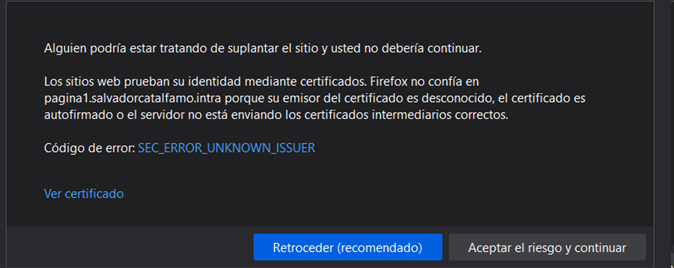
\includegraphics[width=15cm,height=6cm]{adv-2.png}
       \end{center}
       \caption{CA Desconocida}
       \label{figCAdesc}
    \end{figure}
 \end{center}

Luego de establecer en nuestra computadora (particularmente en el navegador Mozilla) que la 
entidad certificante creada es confiable, es posible ver que nuestra conexión es segura, como 
se muestra en la captura.

\begin{center}
    \begin{figure}   
       \begin{center}
          \includegraphics[width=15cm,height=7.5cm]{ca-HTTPS.png}
       \end{center}
       \caption{Resultado de la solución}
    \end{figure}
 \end{center}







\section{Propuesta 3: Certificación con Let's Encrypt}
Esta estrategia consiste en generar un certificado wildcard, y utilizarlo en cada sitio de la organización.
Para esto se debe tener un dominio (en mi caso, salvadorcatalfamo.com) y demostrar la propiedad 
del mismo. Como se vio anteriormente, hay dos maneras que utiliza Let's Encrypt para demostrar la propiedad 
de un dominio, pero la que nos sirve en el caso de una red interna es la que intervienen los registros DNS. 
La verificación que ofrecen con este tipo de certificado es la mínima (DV) y el proceso es explicado a 
continuación.


\subsection{Pasos a seguir}
\subsubsection*{Obtener un dominio}
El primer paso es conseguir un dominio, en mi caso ya tenía uno:
salvadorcatalfamo.com. Este dominio apunta a nuestra ip pública. La configuración DNS
es la siguiente:  


\begin{longtable}{|l|l|p{5cm}|l|l|} 
   \hline
   \textbf{Tipo} & \textbf{Nombre} & \textbf{Contenido} & \textbf{Prioridad} & \textbf{TTL}
\\ \hline A  & salvadorcatalfamo.com & 181.228.121.12 & 0 & 14400
\\ \hline NS  & salvadorcatalfamo.com & ns1.donweb.com & 0 & 14400
\\ \hline SOA & salvadorcatalfamo.com & ns2.donweb.com & 0 & 14400
\\ \hline SOA & salvadorcatalfamo.com & ns3.hostmar.com \newline root.hostmar.com 
                                       \newline 2021010700 28800 7200 
                                       \newline 2000000 86400
                                       \newline ns2.donweb.com & 0 & 14400                  


\\ \hline
\end{longtable}

\subsubsection*{Instalando Let’s Encrypt en el servidor}
\begin{verbatim}
   sudo add-apt-repository ppa:certbot/certbotsudo 
   apt-get update
   sudo apt-get install python-certbot-nginx
\end{verbatim}

\subsubsection*{Instalando Nginx}
\begin{verbatim}
sudo apt-get update
sudo apt-get install nginx
\end{verbatim}


\subsubsection*{Obteniendo un certificado SSL de tipo wildcard desde Let’s Encrypt}
\begin{verbatim}
sudo certbot --server https://acme-v02.api.letsencrypt.org/directory 
-d *.salvadorcatalfamo.com --manual --preferred-challenges dns-01 certonly
\end{verbatim}

\subsubsection*{Configuración DNS}
Luego de ejecutar el comando anterior, Let's Encrypt nos da un contenido que 
se debe agregar a un registro DNS. El tipo de registro es TXT y se muestra en
la siguiente tabla.

\begin{longtable}{|l|l|l|l|l|} 
   \hline
   \textbf{Tipo} & \textbf{Nombre} & \textbf{Contenido} & \textbf{Prioridad} & \textbf{TTL}
\\ \hline TXT  & 	\_acme-challenge.salvadorcatalfamo.com & 11UZJD27bPDb\_jFs6f... & 0 & 14400
\\ \hline
\end{longtable}

\subsubsection*{Configuración de Nginx para servir a subdominios}

Se debe modificar el siguiente archivo de 
configuración 

/etc/nginx/sites-available/salvadorcatalfamo.com como se muestra a 
continuación:

\begin{verbatim}
server {
   listen 80;
   listen [::]:80;
   server_name *.salvadorcatalfamo.com;
   return 301 https://$host$request_uri;
}
server {
   listen 443 ssl;
   server_name *.example.com;  ssl_certificate /.../.../fullchain.pem;
   ssl_certificate_key /.../privkey.pem;
   include /etc/letsencrypt/options-ssl-nginx.conf;
   ssl_dhparam /.../ssl-dhparams.pem;  root /.../salvadorcatalfamo.com;
   index index.html;
   location / {
      try_files $uri $uri/ =404;
   }
} 
\end{verbatim}


\subsubsection*{Test la configuración y reinicio del servicio}

La configuración se puede testear con el siguiente comando: 
\begin{verbatim}
      sudo nginx -t
\end{verbatim}

Si tiene éxito, se debe volver a cargar Nginx usando
\begin{verbatim}
      sudo /etc/init.d/nginx reload
\end{verbatim}

Ahora Nginx contiene un certificado de tipo wildcard, un certificado SSL con respaldo de una 
entidad certificante como Let's Encrypt

\begin{center}
   \begin{figure}   
      \begin{center}
         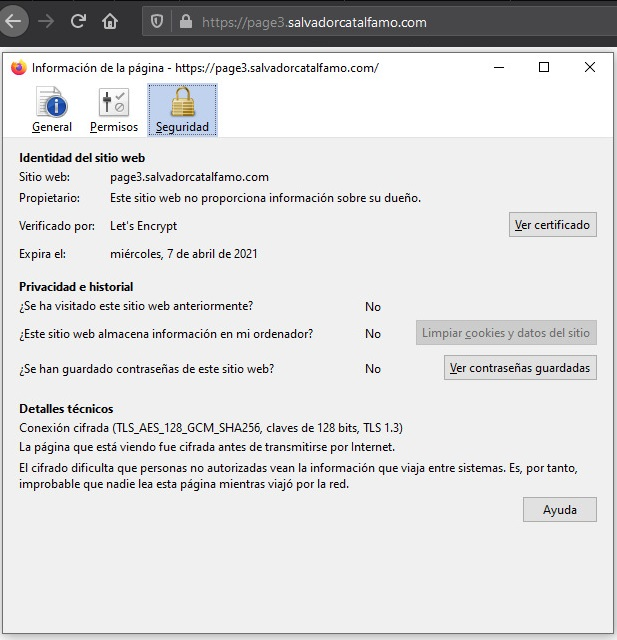
\includegraphics[width=15cm,height=16cm]{lets.png}
      \end{center}
      \caption{Web interna con certificado de Let’s Encrypt}
   \end{figure}
\end{center}

Le hemos visto un gran potencial a esta solución, aunque también es poco implementada. Tenemos la gran ventaja de no
tener que instalar ningún requerimiento en las computadoras dentro de la organización. Con esto, no se 
mostrarán mensajes de seguridad en los navegadores, no importa cuál sea el programa, ya que Let's Encrypt es 
una entidad de confianza para diversos navegadores y sistemas operativos. Todo esto y la seguridad extra al 
saber que nuestros datos van por un canal seguro gracias al protocolo SSL. 

Otra gran ventaja que vimos es la facilidad con la que se llevó a cabo, 
en este proyecto se logró implementar antes esta solución que la entidad certificante, y 
con mucha mayor facilidad. 

Como desventajas podemos decir que no tenemos la posibilidad de obtener la validación extendida (EV), ya que no está
disponible actualmente. Por otro lado, que las llaves privadas y el certificado (que es único para todo el dominio) 
estén en diversos servidores a la vez, implica
que se deben tener mayores recaudos a la hora de utilizarlos, ya que se debe asegurar el control de éstos. Aunque a 
nosotros no nos sucedió, puede llegar a suceder que si se pierde conexión a Internet, el certificado no se pueda validar,
producto de no tener toda la cadena de certificación hasta llegar a la raíz. 

Aunque se puede llegar a pensar, administrar los certificados y las llaves puede llegar a ser 
un gran desafío para los administradores de sistema, sin embargo, hay muchas herramientas que nos proveen
automatización y monitoreo para realizar esta clase de tareas. 


\section{Caso de estudio: Buscando credenciales en tráfico seguro}

Luego de ver las diversas soluciones propuestas, una parte importante de 
nuestro proyecto fue verificar que verdaderamente aumenta la seguridad
cuando nuestro tráfico va encriptado. Para este caso de estudio, se utilizó
el mismo formulario propuesto en la sección \ref{secCaseOfStudy}, lo 
único que con servidores en distintas direcciones.

Dado que el proceso de capturar el tráfico en una red interna fue
explicado previamente, se van a mostrar únicamente los paquetes capturados
desde la primera solicitud hasta el envío del formulario.

\begin{center}
   \begin{figure}   
      \begin{center}
         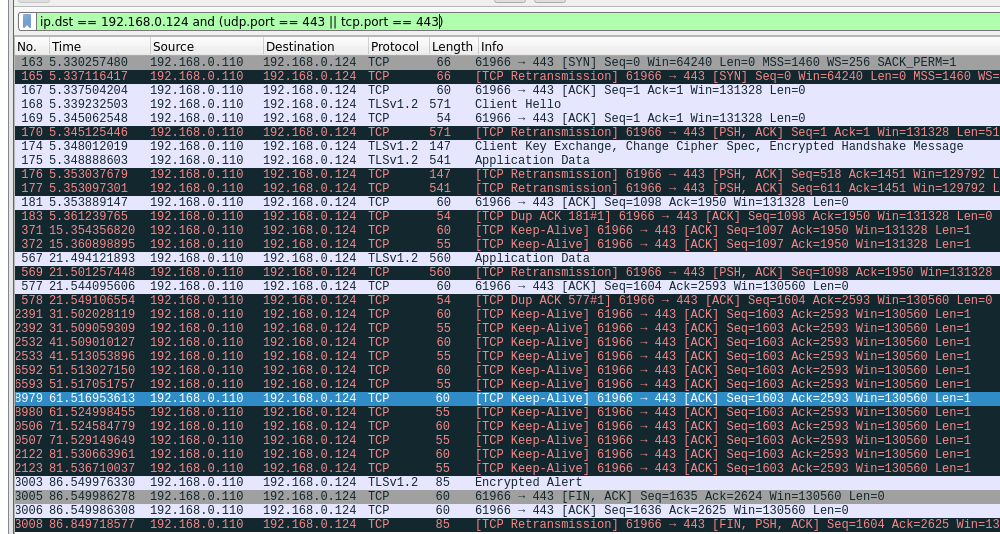
\includegraphics[width=15cm,height=9cm]{verificacion-ssl-1-v2.png}
      \end{center}
      \caption{Tráfico capturado}
   \end{figure}
\end{center}

En esta captura podemos observar que:
\begin{itemize}
   \setlength\itemsep{-0.6em}
   \item No es posible determinar a simple vista cual es el paquete 
   en el cual se envía la información crítica.
   \item Abriendo e investigando el contenido de cada uno de los paquetes mostrados,
   tampoco es posible ver las credenciales completadas en el formulario, 
   que obviamente son de nuestro conocimiento.
   \item Se establece una conexión segura a través del protocolo TCP, algo que no 
   vimos en el caso de estudio de HTTP.
\end{itemize}







% =================================================================== %

\chapter{Conclusiones y Resultados Obtenidos}
    \label{capConc}

%-*- ES -*-
%----------------------------------------------------------------------
% Capitulo 7: Conclusiones generales
%----------------------------------------------------------------------

En este proyecto abordamos una amplia cantidad de temas de manera resumida, con un gran potencial 
de estudio por delante. Aunque en un principio se deseaba investigar todo el tráfico que pasaba por 
la red interna, con todas las posibles debilidades, la navegación web nos permitió encontrar una 
extensa cantidad de nuevos conceptos para desarrollar, tales como los protocolos HTTP, HTTPS, DNS, 
y los posibles procesos que se pueden realizar para segurizar nuestra red.

Con respecto a Docker, no nos resultó muy complejo realizar nuestras tareas, ya que la comunidad 
es muy amplia, y las herramientas que nos brindan están al alcance de nuestra mano. El tiempo que 
nos ahorramos con Docker fue destinado a entender el funcionamiento de la seguridad en las redes, 
tales como el uso de los certificados SSL y las entidades certificantes.

A pesar del contenido teórico propuesto, el trabajo se concentró en las soluciones presentadas 
en el capítulo 4. Allí se explicó brevemente como con un corto conocimiento en el funcionamiento 
del protocolo SSL se pueden establecer mecanismos para que el tráfico web vaya de manera segura; 
uno de nuestros principales objetivos, junto con el de concientizar a las personas de la 
importancia de conocer los sitios por los que se navega. Aunque en nuestro caso abordamos las 
redes pertenecientes a una organización, el contenido de la información es válido para cualquier 
sitio web que se visita, ya sea interno o externo. 


% =================================================================== %

\appendix
\chapter{Glosario}

%-*- ES -*-
\section{Terminolog\'{\i}a}

\begin{longtable}{|l|l|} \hline
\textbf{T\'ermino en ingl\'es} & \textbf{Traducci\'on utilizada}
\\ \hline \hline stateless & sin estado
\\ \hline Secure Sockets Layer & capa de Sockets seguros
\\ \hline wildcard & comodín
\\ \hline framework & sistema
\\ \hline man-in-the-middle & hombre en el medio
\\ \hline Sniffing & olfateo
\\ \hline Spoofing & engañar
\\ \hline Self-signed Certificates & certificados auto-firmados
\\ \hline Namespaces & espacios de nombres  \\ \hline
\end{longtable}




%bibliografia
\bibliography{tesis}
\bibliographystyle{acm}
%\bibliographystyle{alpha}


\end{document}
